%%%%%%%%%%%%%%%%%%%%%%%%%%%%%%%%%%%%%%%%%%%%%%%%%%%%%%%%%%%%%%%%%%%%%%%%%%%%%%%%%%%%%%%%%%
%%%%%%%%%%%%%%%%%%%%%%%%%%%%%%%%%%%%%%%%%%%%%%%%%%%%%%%%%%%%%%%%%%%%%%%%%%%%%%%%%%%%%%%%%%
%%%%%%%%%%%%%%%%%%%%%%%%%%%%%%%%%%%%%%%%%%%%%%%%%%%%%%%%%%%%%%%%%%%%%%%%%%%%%%%%%%%%%%%%%%
\section{Radon Measures}


%%%%%%%%%%%%%%%%%%%%%%%%%%%%%%%%%%%%%%%%%%%%%%%%%%%%%%%%%%%%%%%%%%%%%%%%%%%%%%%%%%%%%%%%%%
\paragraph{Measures.}

We will interchangeably the term histogram or probability vector for any element $\a \in \simplex_n$ that belongs to the probability simplex
\eq{
	\simplex_n \eqdef \enscond{\a \in \RR_+^n}{ \sum_{i=1}^n \a_i = 1 }.
}
A discrete measure with weights $\a$ and locations $x_1,\dots,x_n\in\X$ reads
\eql{\label{eq-discr-meas}
	\al = \sum_{i=1}^n \a_i \de_{x_i}
}
where $\de_x$ is the Dirac at position $x$, intuitively a unit of mass which is infinitely concentrated at location $x$. Such as measure describes a probability measure if, additionally, $\a\in\simplex_n$, and more generally a positive measure if each of the ``weights'' described in vector $\a$ is positive itself. 


\begin{rem}[General measures]
A convenient feature of OT is that it can deal with discrete and continuous ``objects'' within the same framework. Such objects only need to be modelled as measures. This corresponds to the notion of Radon measures $\Mm(\X)$ on the space $\X$. The formal definition of that set 
requires that $\X$ is equipped with a distance, usually denoted $\dist$, because one can only access a measure by ``testing'' (integrating) it against continuous functions, denoted $f \in \Cc(\X)$. 

Integration of $f \in \Cc(\X)$ against a discrete measure $\al$ computes a sum
\eq{ 
	\int_\X f(x) \d\al(x) = \sum_{i=1}^n \a_i f(x_i).
}
%
More general measures, for instance on $\X=\RR^\dims$ (where $\dims \in \NN^*$ is the dimension), can have a density $\d\al(x)=\density{\al}(x)\d x$ w.r.t. the Lebesgue measure, often denoted $\density{\al} = \frac{\d\al}{\d x}$, which means that 
\eq{
	\foralls h \in \Cc(\RR^\dims), \quad
	\int_{\RR^\dims} h(x) \d\al(x) =  \int_{\RR^\dims} h(x) \density{\al}(x) \d x.
}
%
An arbitrary measure $\al \in \Mm(\X)$ (which needs not to have a density nor be a sum of Diracs) is defined by the fact that it can be integrated agains any continuous function $f \in \Cc(\X)$ and obtain $\int_\X f(x) \d\al(x) \in \RR$. If $\X$ is not compact, one should also impose that $f$ has compact support or at least as $0$ limit at infinity. 
%
Measure as thus in some sense ``less regular'' than functions, but more regular than distributions (which are dual to smooth functions). For instance, the derivative of a Dirac is not a measure.
%
We denote $\Mm_+(\X)$ the set of all positive measures on $\X$. The set of probability measures is denoted $\Mm_+^1(\X)$, which means that any $\al \in \Mm_+^1(\X)$ is positive, and that $\al(\X)=\int_\Xx \d\al = 1$. 
%
Figure~\ref{fig-measures} offers a visualization of the different classes of measures, beyond histograms, considered in this work.
\end{rem}


\begin{figure}
\centering
\begin{tabular}{@{}c@{\hspace{1mm}}c@{\hspace{1mm}}c@{\hspace{1mm}}c@{}}
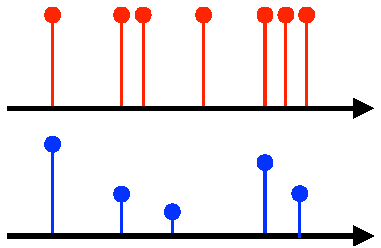
\includegraphics[width=.24\linewidth]{measures/discrete-1d}&
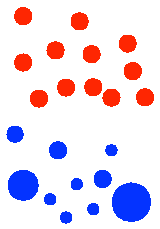
\includegraphics[width=.15\linewidth]{measures/discrete-2d}&
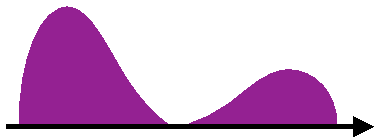
\includegraphics[width=.24\linewidth]{measures/density-1d}&
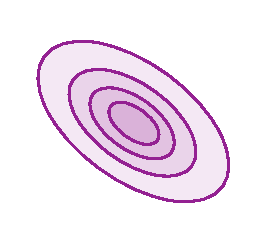
\includegraphics[width=.22\linewidth]{measures/density-2d}\\
Discrete $d=1$ & Discrete $d=2$ & Density $d=1$ & Density $d=2$
\end{tabular}
\caption{\label{fig-measures}
Schematic display of discrete distributions $\al = \sum_{i=1}^n \a_i \de_{x_i}$ (red corresponds to empirical uniform distribution $\a_i=1/n$, and blue to arbitrary distributions) and densities $\d\al(x)=\density{\al}(x)\d x$ (in violet), in both 1-D and 2-D. Discrete distributions in 1-D are displayed using vertical segments (with length equal to $\a_i$) and in 2-D using point clouds (radius equal to $\a_i$). 
}
\end{figure}



%%%%%%%%%%%%%%%%%%%%%%%%%%%%%%%%%%%%%%%%%%%%%%%%%%%%%%%%%%%%%%%%%%%%%%%%%%%%%%%%%%%%%%%%%%
\paragraph{Operators on measures.}


For some continuous map $\T : \X \rightarrow \Y$, we define the pushforward operator $\T_\sharp : \Mm(X) \rightarrow \Mm(Y)$. 
%
For discrete measures~\eqref{eq-discr-meas}, the pushforward operation consists simply in moving the positions of all the points in the support of the measure
\eq{
	\T_{\sharp} \al \eqdef \sum_i \a_i \de_{\T(x_i)}.
}
For more general measures, for instance for those with a density, the notion of push-forward plays a fundamental to describe spatial modifications of probability measures. The formal definition reads as follow.

\begin{defn}[Push-forward]\label{defn-pushfwd}
For $\T : \X \rightarrow \Y$, the push forward measure $\be = \T_\sharp \al \in \Mm(\Y)$ of some $\al \in \Mm(\X)$ reads
\eql{\label{eq-push-fwd}
	\foralls h \in \Cc(\Y), \quad \int_\Y h(y) \d \be(y) = \int_\X h(\T(x)) \d\al(x).
	% = \int_X h(T(x)) \density{\al}(x) \d x %%%% y=T(x)   dy=|T'(x)| dx
	% = \int_Y h(y) \density{\al}(T^{-1}(y)) 1/|T'(x)| \d y 
	% = \int_Y h(y) \density{\be}(y) \d y
	%  \density{\al}(T^{-1}(y)) 1/|T'(x)| = \density{\be}(y)
}
Equivalently, for any measurable set $B \subset \Y$, one has
\eql{\label{eq-equiv-pushfwd}
	\be(B) = \al( \enscond{x \in \X}{\T(x) \in B} ).
}
Note that $\T_\sharp$ preserves positivity and total mass, so that if $\al \in \Mm_+^1(\X)$ then $\T_\sharp \al \in \Mm_+^1(\Y)$. 
\end{defn}

Intuitively, a measurable map $T: \X\rightarrow \Y$, can be interpreted as a function ``moving'' a single point from a measurable space to another. The more general extension $T_\sharp$ can now ``move'' an entire probability measure on $\X$ towards a new probability measure on $\Y$. The operator $T_\sharp$ ``pushes forward'' each elementary mass of a measure $\al$ on $\X$ by applying the map $T$ to obtain then an elementary mass in $\Y$, to build on aggregate a new measure on $\Y)$ written $T_{\sharp}\al$.  Note that such a push-forward $\T_\sharp : \Mm_+^1(\X) \rightarrow \Mm_+^1(\Y)$ is a linear operator between measures in the sense that for two measures $\al_1,\al_2$ on $\X$, $T_\sharp(\al_1+\al_2)=T_\sharp\al_1+ T_\sharp\al_2$.



%%%%%%%
\begin{rem}[Push-forward for densities]
Explicitly doing the change of variable in formula~\eqref{eq-push-fwd} for measures with densities $(\density{\al},\density{\be})$ on $\RR^\dims$ (assuming $\T$ is smooth and a bijection) shows that a push-forward acts on densities linearly as a change of variables in the integration formula, indeed
\eql{\label{eq-pfwd-density}
	\density{\al}(x) = |\det(\T'(x))|  \density{\be}(\T(x))
}
where $\T'(x) \in \RR^{\dims \times \dims}$ is the Jacobian matrix of $T$ (the matrix formed by taking the gradient of each coordinate of $T$).
This implies, denoting $y=\T(x)$
\eq{
	|\det(\T'(x))| = \frac{ \density{\al}(x) }{ \density{\be}(y) }.
}
\end{rem}
%%%%%%%


%%%%%%%
\begin{rem}[Push-forward vs. pull-back]
The push-forward $\T_\sharp$ of measures should not be confounded with the pull-back of function $\T^\sharp : \Cc(\Y) \rightarrow \Cc(\X)$ which corresponds to the ``warping'' of functions. It is the linear map defined, for $g \in \Cc(\Y)$ by $\T^\sharp g = g \circ \T$. Push-forward and pull-back are actually adjoint one from each others, in the sense that
\eq{
	\foralls (\al,g) \in \Mm(\X) \times \Cc(Y), \quad
	\int_\Y g \d( \T_\sharp\al ) = \int_\X (\T^\sharp g) \d\al.
}
It is important to realize that even if $(\al,\be)$ have densities $(\density{\al},\density{\be})$, $\T_\sharp \al$ is not equal to $\T^\sharp \density{\be}$, because of the presence of the Jacobian in~\eqref{eq-pfwd-density}.
%
This explains why OT should be used with caution to perform image registration, because it does not operate as an image warping method.
%
Figure~\ref{fig-push-pull} illustrate the distinction between these push-forward and pull-back operators. 
\end{rem}
%%%%%%%


\begin{figure}
\centering
\begin{tabular}{@{}c@{\hspace{5mm}}c@{}}
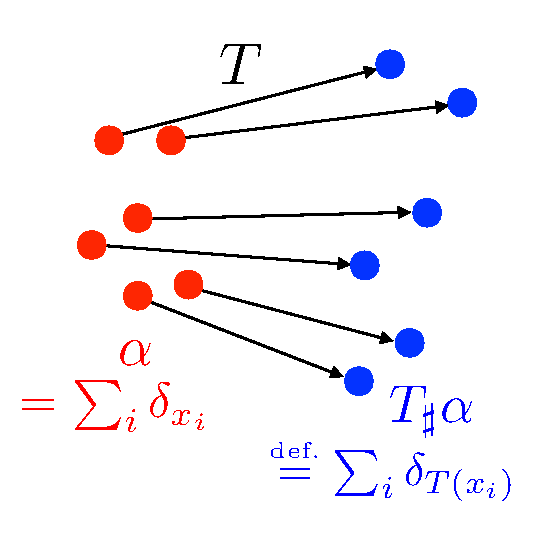
\includegraphics[width=.3\linewidth]{push-pull/push-forward}&
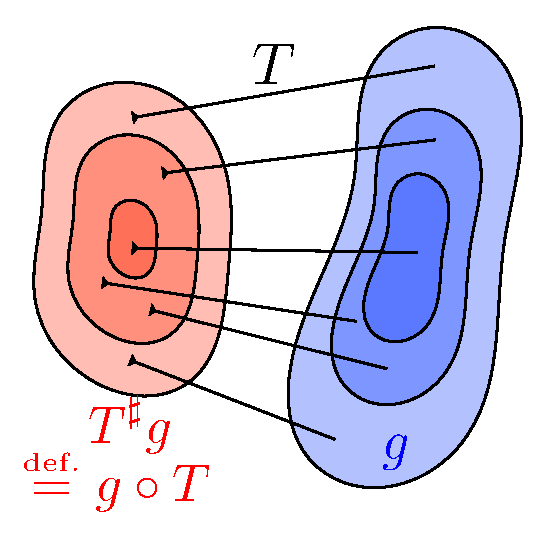
\includegraphics[width=.3\linewidth]{push-pull/pull-back}\\
Push-forward of measures & Pull-back of functions
\end{tabular}
\caption{\label{fig-push-pull}
Comparison of push-forward $\T_\sharp$ and pull-back $\T^\sharp$.
}
\end{figure}



%%%%%%%%%%%%%%
\begin{rem}[Measures and random variables]
	Radon measures can also be viewed as representing the distributions of random variables. A random variable $X$ on $\X$ is actually a map $X : \Om \rightarrow \X$ from some abstract (often un-specified) probabized space $(\Om,\PP)$, and its distribution $\al$ is the Radon measure $X \in \Mm_+^1(\X)$ such that $\PP(X \in A) = \al(A)=\int_A \d\al(x)$.
	%
	Equivalently, it is the push-forward of $\PP$ by $X$, $\al=X_\sharp\PP$.
	%
	Applying another push-forward $\be = \T_\sharp\al$ for $\T : \X \rightarrow \Y$, following~\eqref{eq-push-fwd}, is equivalent to defining another random variable $Y=\T(X) : \om \in \Om \rightarrow \T(X(\om)) \in Y$, so that $\be$ is the distribution of $Y$.
	%
	Drawing a random sample $y$ from $Y$ is thus simply achieved by computing $y=\T(x)$ where $x$ is drawn from $X$.  
\end{rem}
%%%%%%%%%%%%%%


%%%%%%%%%%%%%%%%%%%%%%%%%%%%%%%%%%%%%%%%%%%%%%%%%%%%%%%%%%%%%%%%%%%%%%%%%%%%%%%%%%%%%%%%%%
\paragraph{Convergence of random variable.}

Convergence of random variable (in probability, almost sure, in law), convergence of measures (strong, weak).


%%%%%%%%%%%%%%%%%%%%%%%%%%%%%%%%%%%%%%%%%%%%%%%%%%%%%%%%%%%%%%%%%%%%%%%%%%%%%%%%%%%%%%%%%%
%%%%%%%%%%%%%%%%%%%%%%%%%%%%%%%%%%%%%%%%%%%%%%%%%%%%%%%%%%%%%%%%%%%%%%%%%%%%%%%%%%%%%%%%%%
%%%%%%%%%%%%%%%%%%%%%%%%%%%%%%%%%%%%%%%%%%%%%%%%%%%%%%%%%%%%%%%%%%%%%%%%%%%%%%%%%%%%%%%%%%
\section{Monge Problem}

Given a cost matrix $(\C_{i,j})_{i \in \range{n}, j \in \range{m}}$, assuming $n=m$, the optimal assignment problem seeks for a bijection $\si$ in the set $\Perm(n)$ of permutations of $n$ elements solving
\eql{\label{eq-optimal-assignment}
	\umin{\si \in \Perm(n)} \frac{1}{n}\sum_{i=1}^n \C_{i,\si(i)}.
}
One could naively evaluate the cost function above using all permutations in the set $\Perm(n)$. However, that set has size $n!$, which is gigantic even for small $n$. Consider for instance that such a set has more than $10^{100}$ elements~\cite{Dantzig1983} when $n$ is as small as 70. That problem can therefore only be solved if there exist efficient algorithms to optimize that cost function over the set of permutations, which will be the subject of~\S\ref{s-matching}.

\begin{rem}[Uniqueness] Note that the optimal assignment problem may have several optimal solutions. Suppose for instance that $n=m=2$ and that the matrix $\C$ is the pairwise distance matrix between the 4 corners of a 2-dimensional square of side length $1$, as represented in the left plot in Figure~\ref{fig-non-unique-matching}. In that case only two assignments exist, and they share the same cost.
\end{rem}

	
\begin{figure}
\centering
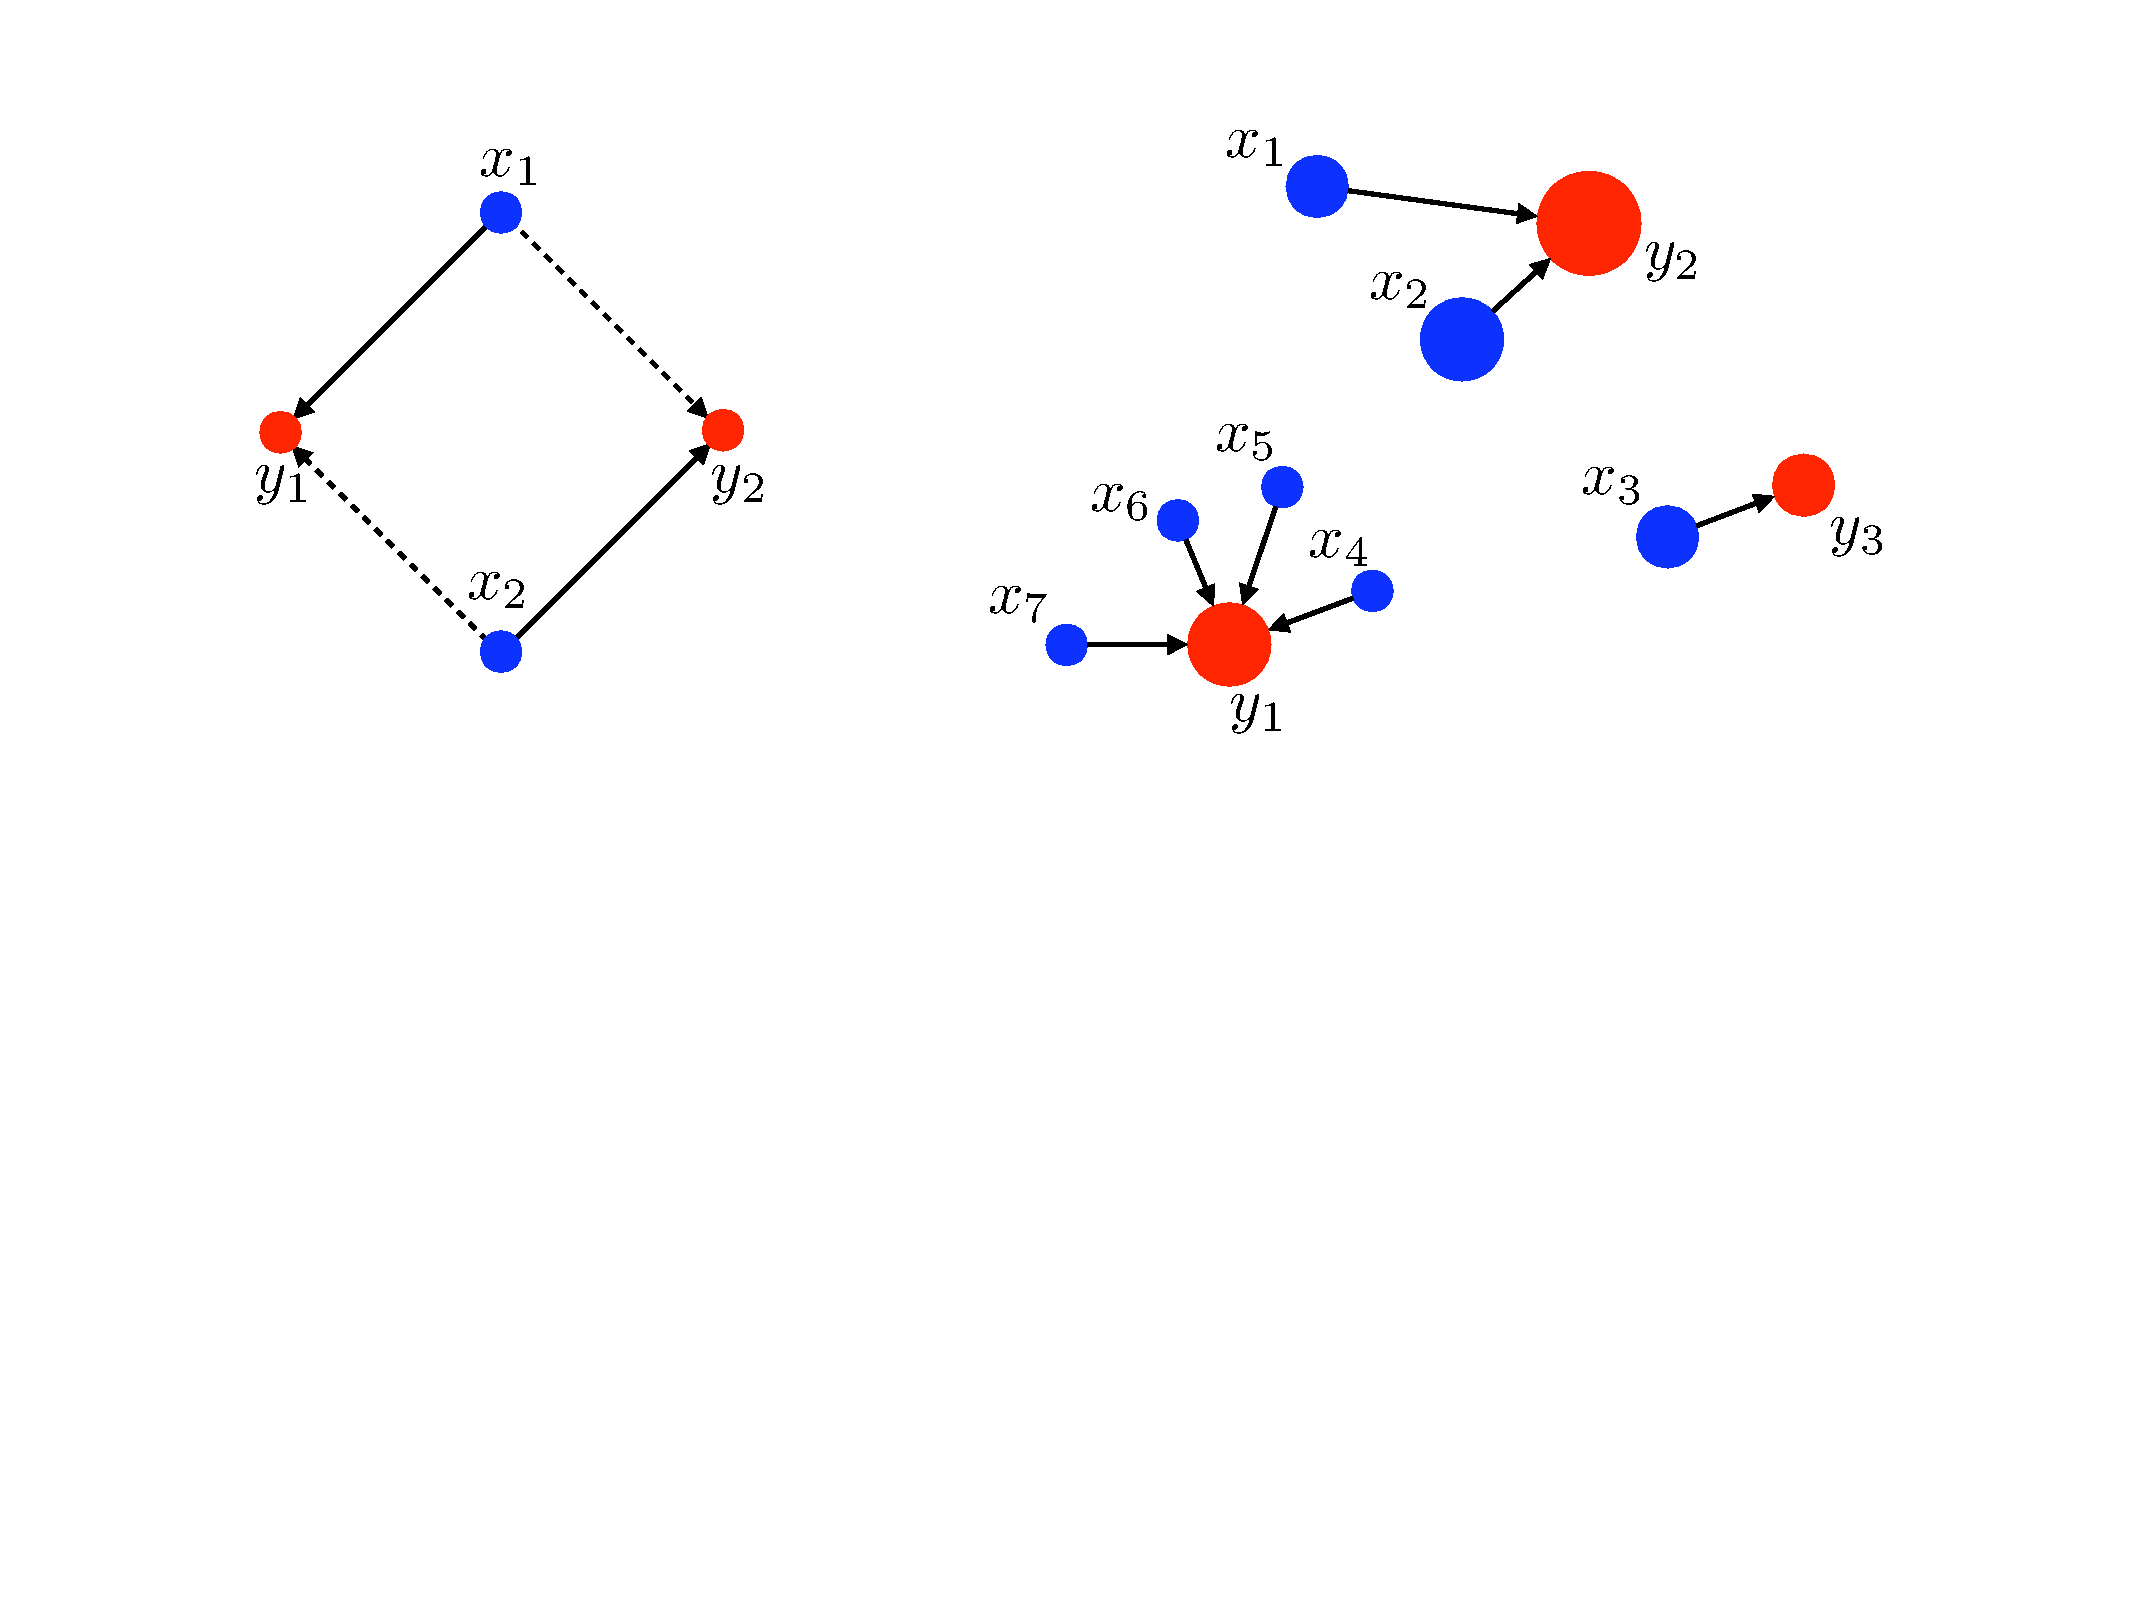
\includegraphics[width=.5\linewidth]{non-unique-optimal-matching/non-unique-optimal-matching}
\caption{\label{fig-non-unique-matching}
(left) blue dots from measure $\alpha$ and red dots from measure $\beta$ are pairwise equidistant. Hence, either matching $\sigma=(1,2)$ (full line) or $\sigma=(2,1)$ (dotted line) is optimal. (right) a Monge map can associate the blue measure $\alpha$ to the red measure $\beta$. The weights $\alpha_i$ are displayed proportionally to the area of the disk marked at each location. The mapping here is such that $T(x_1)=T(x_2)=y_2$, $T(x_3)=y_3$, whereas for $4\leq i\leq 7$ we have $T(x_i)=y_1$.
}
\end{figure}

For discrete measures 
\eql{\label{eq-pair-discr}
	\al = \sum_{i=1}^n \a_i \de_{x_i}
	\qandq
	\be = \sum_{j=1}^m \b_j \de_{y_j}
}
the Monge problem~\cite{Monge1781} seeks for a map that associates to each point $x_i$ a single point $y_j$, and which must push the mass of $\al$ toward the mass of $\be$, which is to say that such a map $T:\{x_1,\dots, x_n\}\rightarrow \{y_1,\dots,y_m\}$ must verify that
\eql{\label{eq-monge-constr}
	\foralls j \in \range{m}, \quad
	\b_j = \sum_{ i : \T(x_i) = y_j } \a_i 
}
which we write in compact form  as $\T_\sharp \al = \be$. 
%
This map should minimize some transportation cost, which is parameterized by a function $\c(x,y)$ defined for points $(x,y) \in \X \times \Y$
\eql{\label{eq-monge-discr}
	\umin{\T} \enscond{ \sum_{i} \c(x_i,\T(x_i))  }{ \T_\sharp \al = \be } .
}
Such a map between discrete points can be of course encoded, assuming all $x$'s and $y$'s are distinct, using indices $\si : \range{n} \rightarrow \range{m}$ so that $j=\si(i)$, and the mass conservation is written as
\eq{
	\sum_{i \in \si^{-1}(j)} \a_i = \b_j.
}
In the special case when $n=m$ and all weights are uniform, that is $\a_i=\b_j=1/n$, then the mass conservation constraint implies that $\T$ is a bijection, such that $\T(x_i)=y_{\si(i)}$, and the Monge problem is equivalent to the optimal matching problem~\eqref{eq-optimal-assignment} where the cost matrix is 
\eq{
	\C_{i,j} \eqdef \c(x_i,y_j). 
}
When $n\ne m$, note that, optimality aside, Monge maps may not even exist between an empirical measure to another. This happens when their weight vectors are not compatible, which is always the case when the target measure has more points than the source measure. For instance, the right plot in Figure~\ref{fig-non-unique-matching} shows an (optimal) Monge map between $\al$ and $\be$, but there is no Monge map from $\be$ to $\al$.


Monge problem~\eqref{eq-monge-discr} is extended to the setting of two arbitrary probability measures $(\al,\be)$ on two spaces $(\X,\Y)$ as finding a map $\T : \X \rightarrow \Y$ that minimizes
\eql{\label{eq-monge-continuous}
	\umin{\T} \enscond{ \int_{\X} \c(x,\T(x)) \d \al(x)  }{  \T_\sharp \al = \be }
}
The constraint $\T_\sharp \al = \be$ means that $\T$ pushes forward the mass of $\al$ to $\be$, and makes use of the push-forward operator~\eqref{eq-push-fwd}. 


%%%%%%%%%%%%%%%%%%%%%%%%%%%%%%%%%%%%%%%%%%%%%%%%%%%%%%%%%%%%%%%%%%%%%%%%%%%%%%%%%%%%%%%%%%
%%%%%%%%%%%%%%%%%%%%%%%%%%%%%%%%%%%%%%%%%%%%%%%%%%%%%%%%%%%%%%%%%%%%%%%%%%%%%%%%%%%%%%%%%%
%%%%%%%%%%%%%%%%%%%%%%%%%%%%%%%%%%%%%%%%%%%%%%%%%%%%%%%%%%%%%%%%%%%%%%%%%%%%%%%%%%%%%%%%%%
\section{Kantorovitch Problem}

The assignment problem has several limitations in practical settings, also encountered when using the Monge problem. Indeed, because the assignment problem is formulated as a permutation problem, it can only be used to compare two points clouds of the \emph{same} size. A direct generalization to discrete measures with non-uniform weights can be carried out using Monge's formalism of pushforward maps, but that formulation may also be degenerate it there does not exist feasible solutions satisfying the mass conservation constraint~\eqref{eq-monge-constr} (see the end of Remark~\ref{rem-monge1}). Additionally, the assignment Problem~\eqref{eq-monge-discr} is combinatorial, whereas the feasible set for the Monge Problem~\eqref{eq-monge-continuous}, consisting in all push-forward measures that satisfy the mass conservation constraint, is \emph{non-convex}. Both are therefore difficult to solve in their original formulation.


%%%%%%%%%%%%%%%%%%%%%%%%%%%%%%%%%%%%%%%%%%%%%%%%%%%%%%%%%%%%%%%%%%%%%%%%%%%%%%%%%%%%%%%%%%
\paragraph{Kantorovitch formulation for discrete measures.}

The key idea of~\cite{Kantorovich42} is to relax the deterministic nature of transportation, namely the fact that a source point $x_i$ can only be assigned to another, or transported to one and one location $T(x_i)$ only. Kantorovich proposes instead that the mass at any point $x_i$ be potentially dispatched across several locations. Kantorovich moves away from the idea that mass transportation should be ``deterministic'' to consider instead a ``probabilistic'' (or ``fuzzy'') transportation, which allows what is commonly known now as ``mass splitting'' from a source towards several targets. This flexibility is encoded using, in place of a permutation $\sigma$ or a map $T$, a coupling matrix $\P  \in \RR_+^{n \times m}$, where $\P_{i,j}$ describes the amount of mass flowing from bin $i$ (or point $x_i$) towards bin $j$ (or point $x_j$), 
$x_i$ towards $y_j$ in the formalism of discrete measures~\eqref{eq-pair-discr}. Admissible couplings admit a far simpler characterization than Monge maps:
\eql{\label{eq-discr-couplings}
	\CouplingsD(\a,\b) \eqdef \enscond{ \P \in \RR_+^{n \times m} }{
		\P \ones_m = \a \qandq 
		\transp{\P} \ones_n = \b	
	},
}
where we used the following matrix-vector notation
\eq{
	\P \ones_m = \left(\sum_j \P_{i,j}\right)_i \in \RR^n
	\qandq
	\transp{\P} \ones_n = \left(\sum_i \P_{i,j}\right)_j \in \RR^m. 
}
The set of matrices $\CouplingsD(\a,\b)$ is bounded, defined by $n+m$ equality constraints, and therefore a convex polytope (the convex hull of a finite set of matrices).

%
Additionally, whereas the Monge formulation (as illustrated in the right plot of Figure~\ref{fig-non-unique-matching}) was intrisically asymmetric, Kantorovich's relaxed formulation is always symmetric, in the sense that a coupling $\P$ is in  $\CouplingsD(\a,\b)$ if and only if  $\transp{\P}$ is in $\CouplingsD(\b,\a)$.

Kantorovich's optimal transport problem now reads
\eql{\label{eq-mk-discr}
	\MKD_{\C}(\a,\b) \eqdef 
	\umin{\P \in \CouplingsD(\a,\b)}
		\dotp{\C}{\P} \eqdef \sum_{i,j} \C_{i,j} \P_{i,j}. 
}
This is a linear program (see Chapter~\ref{c-algo-basics}), and as is usually the case with such programs, its solutions are not necessarily unique. 



%%%%%%%%%%%%%%%%%%%%%%%%%%%%%%%%%%%%%%%%%%%%%%%%%%%%%%%%%%%%%%%%%%%%%%%%%%%%%%%%%%%%%%%%%%
\paragraph{Permutation Matrices as Couplings} 

For a permutation $\si\in\Perm(n)$, we write $\P_{\si}$ for the corresponding permutation matrix,
	\eql{\label{eq-perm-matrices}
		\foralls (i,j) \in \range{n}^2, \quad
		(\P_{\si})_{i,j} = \choice{
			1/n \qifq j=\si_i, \\
			0 \quad\text{otherwise.} 
		}
	} 
One can check that in that case
\eq{\dotp{\C}{\P_{\si}}=\frac{1}{n}\sum_{i=1}^n \C_{i,\si_i},}
which shows that the assignment problem~\eqref{eq-optimal-assignment} can be recast as a Kantorovich problem~\eqref{eq-mk-discr} where the couplings $\P$ are restricted to be exactly permutation matrices:
\eq{\umin{\si \in \Perm(n)} \frac{1}{n}\sum_{i=1}^n \C_{i,\si(i)} = \umin{\si \in \Perm(n)} \dotp{\C}{\P_{\si}}.}
Next, one can easily check that the set of permutation matrices is strictly included in the so-called Birkhoff polytope $\CouplingsD(\ones_n/n,\ones_n,n)$. Indeed, for any permutation $\si$ we have $\P_{\si}\ones=\ones_n$ and $\transp{\P_{\si}}\ones=\ones_n$, whereas $\ones_n\transp{\ones_n}/n^2$ is a valid coupling but not a permutation matrix. Therefore, one has naturally that
$$ \umin{\si \in \Perm(n)} \dotp{\C}{\P_{\si}} \leq  \MKD_{\C}(\ones_n/n,\ones_n/n).$$

The following proposition shows that these problems result in fact in the same optimum, namely that one can always find a permutation matrix that minimizes Kantorovich's problem~\eqref{eq-mk-discr} between two uniform measures $\a=\b=\ones_n/n$, which shows that the Kantorovich relaxation is \emph{tight} when considered on assignment problems. %Note however that some computational algorithm, which are combinatorial in nature, are dedicated to the case of uniform histograms with the same number of points (see Chapter~\ref{c-algo-basics}). 
%
Figure~\ref{fig-matching-kantorovitch} shows on the left a 2-D example of optimal matching corresponding to this special case. 
%

\begin{figure}
\centering
\begin{tabular}{@{}c@{\hspace{5mm}}c@{}}
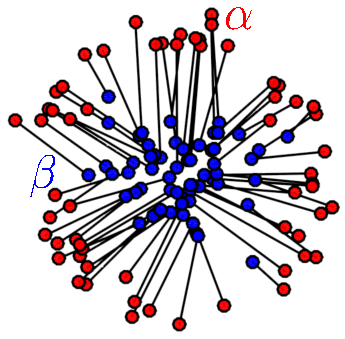
\includegraphics[width=.25\linewidth]{matching-kantorovitch/matching}&
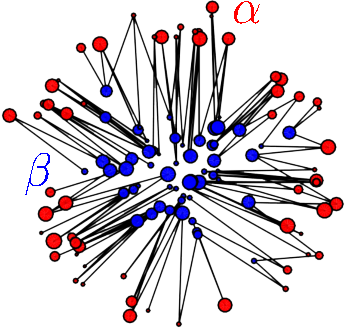
\includegraphics[width=.25\linewidth]{matching-kantorovitch/weighted}
\end{tabular}
\caption{\label{fig-matching-kantorovitch}
%
Comparison of optimal matching and generic couplings. A black segment between $x_i$ and $y_j$ indicates a non-zero element in the displayed optimal coupling $\P_{i,j}$ solving~\eqref{eq-mk-discr}.
%
Left: optimal matching, corresponding to the setting of Proposition~\eqref{prop-matching-kanto} (empirical measures with the same number $n=m$ of points).
%
Right: these two weighted point clouds cannot be matched; instead a Kantorovich coupling can be used to associate two arbitrary discrete measures.  
}
\end{figure}


\begin{prop}[Kantorovich for matching]\label{prop-matching-kanto}
	If $m=n$ and $\a=\b=\ones_n/n$, then there exists an optimal solution for Problem~\eqref{eq-mk-discr} $\P_{\si^\star}$, which is a permutation matrix associated to an optimal permutation $\si^\star \in \Perm(n)$ for Problem~\eqref{eq-optimal-assignment}.	
\end{prop}

\begin{proof}
	Birkhoff's theorem states that the set of extremal points of $\CouplingsD(\ones_n/n,\ones_n/n)$ is equal to the set of permutation matrices. A fundamental theorem of linear programming
	\cite[Theorem 2.7]{bertsimas1997introduction} 
	states that the minimum of a linear objective in a non-empty polyhedron, if finite, is reached at an extremal point of the polyhedron.
\end{proof}




%%%%%%%%%%%%%%%%%%%%%%%%%%%%%%%%%%%%%%%%%%%%%%%%%%%%%%%%%%%%%%%%%%%%%%%%%%%%%%%%%%%%%%%%%%
\paragraph{Kantorovitch formulation for arbitrary measures.}


The definition of $\MK_\c$ in~\eqref{eq-kanto-discr} can be extended to arbitrary measures by considering couplings $\pi \in \Mm_+^1(\X \times \Y)$ which are joint distributions over the product space. The discrete case is a special situation where one imposes this product measure to be of the form $\pi = \sum_{i,j} \P_{i,j} \de_{(x_i,y_j)}$. In the general case, the mass conservation constraint~\eqref{eq-discr-couplings} should be rewritten as a marginal constraint on joint probability distributions
\eql{\label{eq-coupling-generic}
	\Couplings(\al,\be) \eqdef 
	\enscond{
		\pi \in \Mm_+^1(\X \times \Y)
	}{
		P_{\X\sharp} \pi = \al
		\qandq
		P_{\Y\sharp} \pi = \be
	}.
} 
Here $P_{\X\sharp}$ and $P_{\Y\sharp}$ are the push-forward (see Definition~\ref{defn-pushfwd}) by the projections $P_\X(x,y)=x$ and $P_\Y(x,y)=y$.
%
Figure~\ref{fig-settings} shows a schematic visualization of the coupling constraints for different class of problem (discrete measures and densities).
%
Using~\eqref{eq-equiv-pushfwd}, these marginal constraints are equivalent to imposing that $\pi(A \times \Y)=\al(A)$ and $\pi(\X \times B)=\be(B)$ for sets $A \subset \X$ and $B \subset \Y$.


\begin{figure}
\centering
\begin{tabular}{@{}c@{\hspace{5mm}}c@{\hspace{5mm}}c@{}}
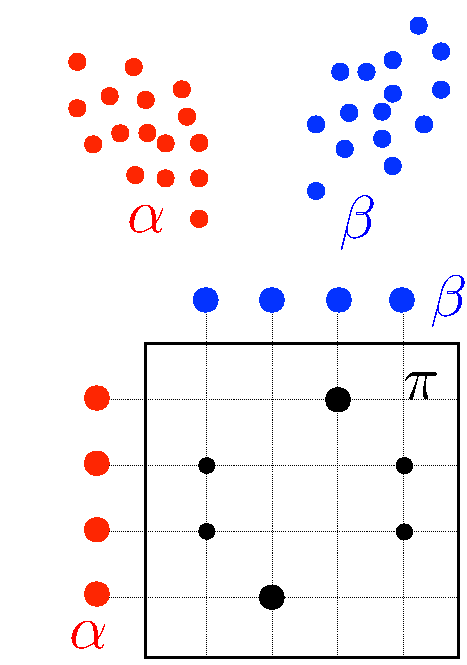
\includegraphics[width=.22\linewidth]{settings/discrete}&
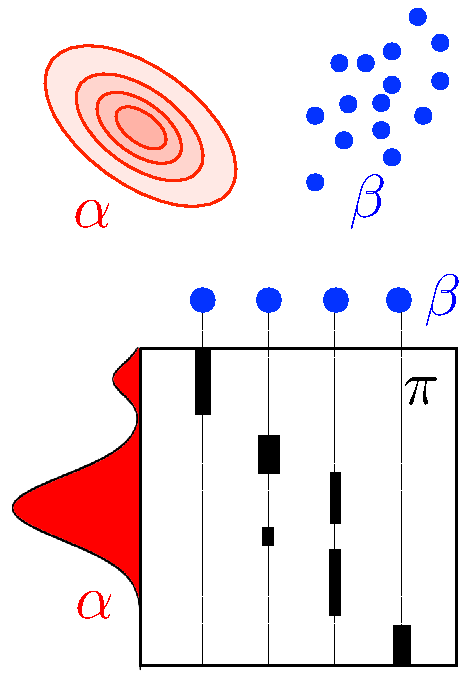
\includegraphics[width=.22\linewidth]{settings/semi-discrete}&
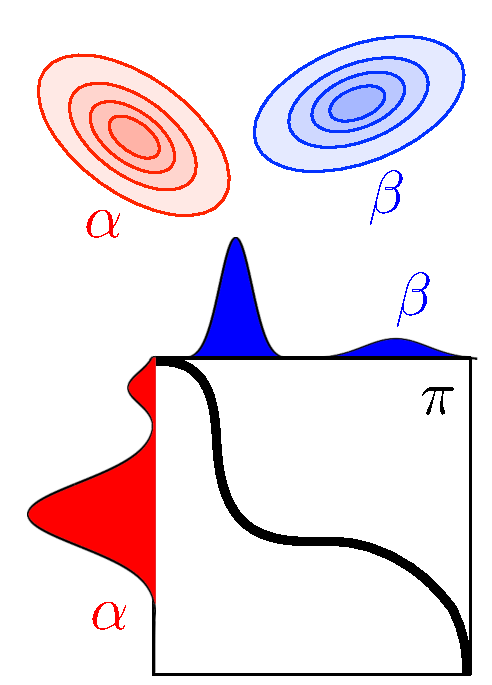
\includegraphics[width=.22\linewidth]{settings/continuous}\\
Discrete & Semi-discrete & Continuous
\end{tabular}
\caption{\label{fig-settings}
Schematic viewed of input measures $(\al,\be)$ and couplings $\Couplings(\al,\be)$ encountered in the three main scenario for Kantorovich OT. Chapter~\ref{c-algo-semidiscr} is dedicated to the semi-discrete setup.
}
\end{figure}



The Kantorovich problem~\eqref{eq-mk-discr} is then generalized as 
\eql{\label{eq-mk-generic}
	\MK_\c(\al,\be) \eqdef 
	\umin{\pi \in \Couplings(\al,\be)}
		\int_{\X \times \Y} \c(x,y) \d\pi(x,y).
}
This is an infinite-dimensional linear program over a space of measures. 
%
Figure~\ref{fig-couplings} shows examples of discrete and continuous optimal coupling solving~\eqref{eq-mk-generic}.
%
Figure~\ref{fig-couplings-simple} shows other examples of optimal 1-D couplings, involving discrete and continuous marginals.



\begin{figure}
\centering
\begin{tabular}{@{}c@{\hspace{10mm}}c@{}}
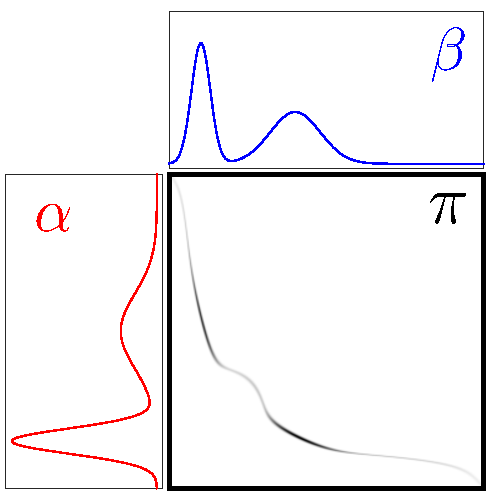
\includegraphics[width=.2\linewidth]{couplings/couplings-continuous}&
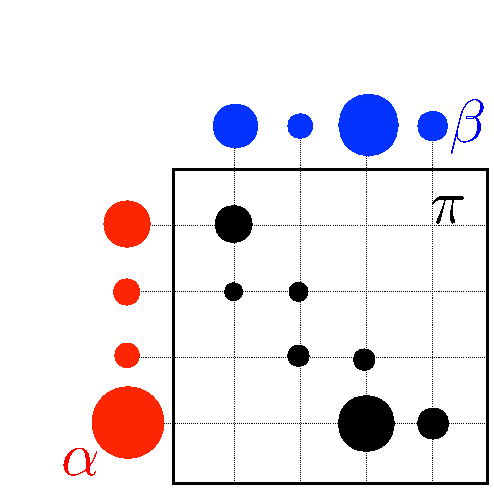
\includegraphics[width=.2\linewidth]{couplings/couplings-discr}
\end{tabular}
\caption{\label{fig-couplings}
Left: ``continuous'' coupling $\pi$ solving~\eqref{eq-coupling-generic} between two 1-D measure with density. The coupling is localized along the graph of the Monge map $(x,\T(x))$ (displayed in black).  
%
Right: ``discrete'' coupling $\T$ solving~\eqref{eq-mk-discr} between two discrete measures of the form~\eqref{eq-pair-discr}. The non-zero entries $\T_{i,j}$  are display with a black disk at position $(i,j)$ with radius proportional to $\T_{i,j}$.
}
\end{figure}


\begin{figure}
\centering
\begin{tabular}{@{}c@{}c@{}c@{}c@{}}
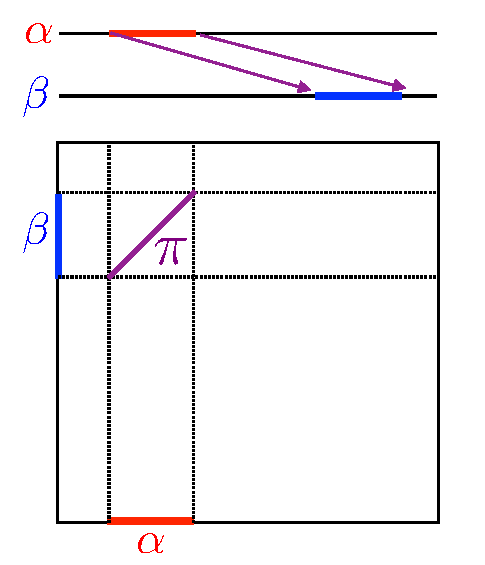
\includegraphics[width=.2\linewidth]{couplings/couplings-1}&
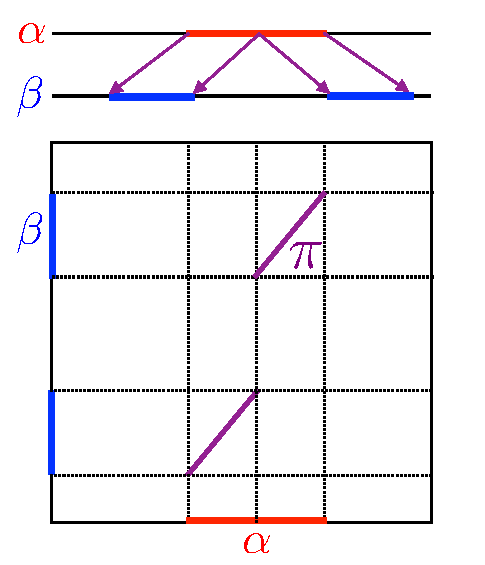
\includegraphics[width=.2\linewidth]{couplings/couplings-2}&
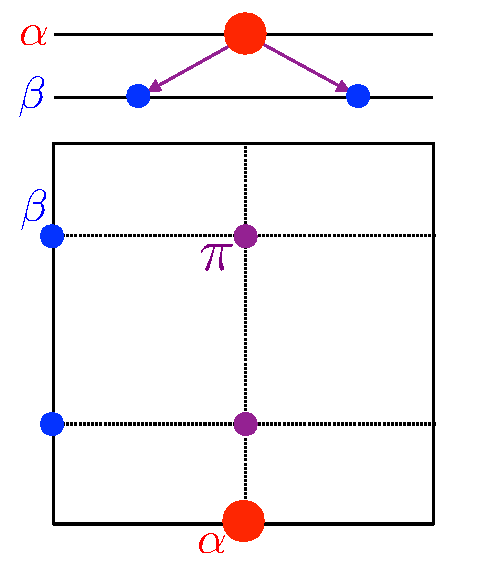
\includegraphics[width=.2\linewidth]{couplings/couplings-3}&
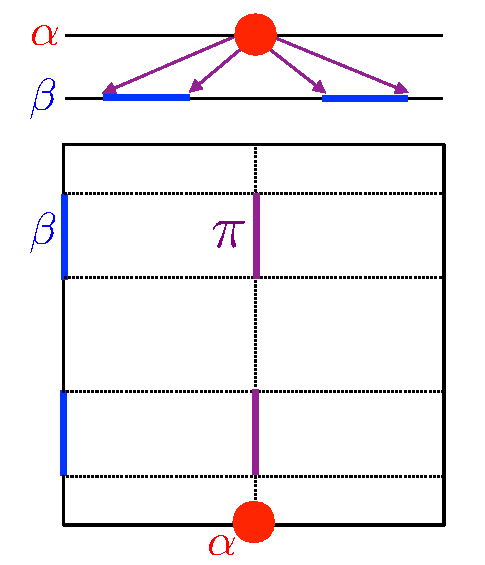
\includegraphics[width=.2\linewidth]{couplings/couplings-4}
\end{tabular}
\caption{\label{fig-couplings-simple}
Four simple examples of optimal couplings between 1-D distributions, represented as maps above (arrows) and couplings below. Inspired by~\cite{Levy2017review}.
}
\end{figure}


On compact domain $(\Xx,\Yy)$, \eqref{eq-mk-generic} always has a solution, because using the weak-* topology (so called weak topology of measures), the set of measure is compact, and a linear function with a continuous $c(x,y)$ is weak-* continuous. And the set of constraint is non empty, taking $\al \otimes \be$. On non compact domain, needs to impose moment condition on $\al$ and $\be$.

% Link with Monge: Brenier theorem (see later using duality). Gradient of convex function. Application for Gaussians. Monge Ampère PDE. 


%%%%%%%%%%%%%%%%%%%%%%%%%%%%%%%%%%%%%%%%%%%%%%%%%%%%%%%%%%%%%%%%%%%%%%%%%%%%%%%%%%%%%%%%%%
\paragraph{Wasserstein distances.}

An important feature of OT is that it defines a distance between histograms and probability measures as soon as the cost matrix satisfies certain suitable properties. Indeed, OT can be understood as a canonical way to lift a ground distance between points to a distance between histogram or measures. 

We first consider the case where, using a term first introduce by~\cite{RubTomGui00}, the ``ground metric'' matrix $\C$ is fixed, representing substitution costs between bins, and shared across several histograms we would like to compare. The following proposition states that OT provides a meaningful distance between histograms supported on these bins.

\begin{prop}\label{prop-metric-histo}
We suppose $n=m$, and that for some $p \geq 1$, $\C=\distD^p=(\distD_{i,j}^p)_{i,j} \in \RR^{n \times n}$ where $\distD \in \RR_+^{n \times n}$ is a distance on $\range{n}$, \emph{i.e.}
\begin{enumerate}% [label=(\roman*)]
	\item $\distD \in \RR_+^{n \times n}$ is symmetric; 
	\item $\distD_{i,j}=0$ if and only if $i=j$; 
	\item $\foralls (i,j,k) \in \range{n}^3, \distD_{i,k} \leq \distD_{i,j}+\distD_{j,k}$.
\end{enumerate}
Then 
\eql{\label{eq-wass-p-disc}
	\WassD_p(\a,\b) \eqdef \MKD_{\distD^p}(\a,\b)^{1/p}
}
(note that $\WassD_p$ depends on $\distD$) defines the $p$-Wasserstein distance on $\Si_n$, \emph{i.e.} $\WassD_p$ is symmetric, positive, $\WassD_p(\a,\b)=0$ if and only if $\a = \b$, and it satisfies the triangle inequality
\eq{
	\foralls \a,\a',\b \in \Si_n, \quad \WassD_p(\a,\b) \leq \WassD_p(\a,\a') + \WassD_p(\a',\b).
}
\end{prop}

\begin{proof}
Symmetry and definiteness of the distance are easy to prove: since $\C = \distD^p$ has a null diagonal, $\WassD_p(\a,\a)=0$, with corresponding optimal transport matrix $\P^\star=\diag(\a)$; by the positivity of all off-diagonal elements of $\distD^p$, $\WassD_p(\a,\b)>0$ whenever $\a\ne \b$ (because in this case, an admissible coupling necessarily has a non-zero element outside the diagonal); by symmetry of $\distD^p$, $\WassD_p(\a,\b)=0$ is itself a symmetric function. 


To prove the triangle inequality of Wasserstein distances for arbitrary measures, \cite[Theorem 7.3]{Villani03} uses the gluing lemma, which stresses the existence of couplings with a prescribed structure. 
% Closed forms for such couplings exist in the discrete case which we can readily use. 
In the discrete setting, the explicit constuction of this glued coupling is simple.
%
Let $\a,\b,\VectMode{c} \in\simplex_n$. Let $\P$ and $\Q$ be two optimal solutions of the transport problems between $\a$ and $\b$, and $\b$ and $\VectMode{c}$ respectively. 
%
We define $\bar\b_j \eqdef \b_j$ if $\b_j>0$ and set otherwise $\bar\b_j=1$ (or actually any other value). We then define 
\eq{
	\SS \eqdef \P \diag(1/\bar\b) \Q \in \RR_+^{n \times n}.
} 
We remark that $\SS \in \U(\a,\VectMode{c})$ because 
\eq{
	\SS \ones_n  = \P \diag(1/\bar\b) \Q \ones_n = \P (\b / \bar\b) = \P \ones_{\Supp(\b)} = \a
}
where we denoted $\ones_{\Supp(\b)}$ the indicator of the support of $\b$, and we use the fact that $\P \ones_{\Supp(\b)} = \P \ones = \b$ because necessarily $\P_{i,j} = 0$ for $j \notin \Supp(\b)$.
Similarly one verifies that $\SS^\top \ones_n = \VectMode{c}$.


The triangle inequality follows from
%   notice that $\SS_{i\cdot k}$ being therefore a matrix of $\U(\a,\b)$ we can write:
$$\begin{aligned}
\WassD_p(\a,\VectMode{c})&=\left(\min_{\P\in U(\a,\VectMode{c})}\dotp{\P}{\distD^p}\right)^{1/p} \leq \dotp{\SS}{\distD^p}^{1/p}\\
&= \left(\sum_{ik} \distD^p_{ik}\sum_{j} \frac{\P_{ij}\Q_{jk}}{\bar\b_j}\right)^{1/p} \leq \left(\sum_{ijk} \left(\distD_{ij}+\distD_{jk}\right)^p \frac{\P_{ij}\Q_{jk}}{\bar\b_j}\right)^{1/p} \\
& \leq \left(\sum_{ijk} \distD^p_{ij} \frac{\P_{ij}\Q_{jk}}{\bar\b_j}\right)^{1/p} + \left(\sum_{ijk}\distD^p_{jk} \frac{\P_{ij}\Q_{jk}}{\bar\b_j}\right)^{1/p} \\
&= \left(\sum_{ij} \distD^p_{ij}\P_{ij} \sum_k \frac{\Q_{jk}}{\bar\b_j}\right)^{1/p} + \left(\sum_{jk} \distD^p_{jk} \Q_{jk} \sum_i \frac{\P_{ij}}{\bar\b_j}\right)^{1/p}\\
&= \left(\sum_{ij} \distD^p_{ij}\P_{ij}\right)^{1/p} + \left(\sum_{jk} \distD^p_{jk} \Q_{jk}\right)^{1/p}\\ 
&= \WassD_p(\a,\b) +\WassD_p(\b,\b).
\end{aligned}
$$
%
The first inequality is due to the suboptimality of $\SS$, the second is the usual triangle inequality for elements in $\distD$, and the third comes from Minkowski's inequality.
\end{proof}

Proposition~\ref{prop-metric-histo} generalizes from histogram to arbitrary measures that need not be discrete.

\begin{prop}\label{prop-metric-measure}
We assume $\X=\Y$, and that for some $p \geq 1$, $\c(x,y)=\dist(x,y)^p$ where $\dist$ is a distance on $\X$, \emph{i.e.} \\
	\hbox{}\qquad (i) $\dist(x,y) = \dist(y,x) \geq 0$;  \\
	\hbox{}\qquad (ii)  $\dist(x,y)=0$ if and only if $x=y$;  \\
	\hbox{}\qquad (ii)  $\foralls (x,y,z) \in \X^3, \dist(x,z) \leq \dist(x,y)+\dist(y,z)$. \\
Then 
\eql{\label{eq-defn-wass-dist}
	\Wass_p(\al,\be) \eqdef \MK_{\dist^p}(\al,\be)^{1/p}
}
(note that $\Wass_p$ depends on $\dist$) defines the $p$-Wasserstein distance on $\X$, \emph{i.e.} $\Wass_p$ is symmetric, positive, $\Wass_p(\al,\be)=0$ if and only if $\al = \be$, and it satisfies the triangle inequality
\eq{
	\foralls (\al,\be,\ga) \in  \Mm_+^1(\X)^3, \quad \Wass_p(\al,\ga) \leq \Wass_p(\al,\be) + \Wass_p(\be,\ga).
}
\end{prop}

\begin{proof}
The proof follows the same approach as that for Proposition~\ref{prop-metric-histo} and relies on the existence of a coupling between $(\al,\ga)$ obtained by ``guying'' optimal couplings between $(\al,\be)$ and $(\be,\ga)$.
\end{proof}

The Wasserstein distance $\Wass_p$ has many important properties, the most important one being that it is a weak distance, \emph{i.e.} it allows to compare singular distributions (for instance discrete ones) and to quantify spatial shift between the supports of the distributions. 
%
In particular, ``classical'' distances (or divergences) are not even defined between discrete distributions (the $L^2$ norm can only be applied to continuous measures with a density with respect to a base measure, and the discrete $\ell^2$ norm requires the positions $(x_i,y_j)$ to be fixed to work). In sharp contrast, one has that for any $p> 0$, $\Wass_p^p(\de_x,\de_y) = \dist(x,y)$. Indeed, it suffices to notice that $\Couplings(\de_x,\de_y)=\{ \delta_{x,y}\}$ and therefore the Kantorovich problem having only one feasible solution, $\Wass_p^p(\de_x,\de_y)$ is necessarily $(\dist(x,y)^p)^{1/p}=\dist(x,y)$. This shows that $\Wass_p(\de_x,\de_y) \rightarrow 0$ if $x \rightarrow y$. 
%
This property corresponds to the fact that $\Wass_p$ is a way to quantify the weak convergence as we now define. 

\begin{defn}[Weak convergence]\label{dfn-weak-conv}
	$(\al_k)_k$ converges weakly to $\al$ in $\Mm_+^1(\Xx)$ (denoted $\al_k \rightharpoonup \al$) if and only if for any continuous function $g \in \Cc(\Xx)$, $\int_\Xx g \d\al_k \rightarrow \int_\Xx g \d\al$.
	%
	This notion of weak convergence corresponds to the convergence in law of random vectors. 
\end{defn}

This convergence can be shown to be equivalent to $\Wass_p(\al_k,\al) \rightarrow 0$~\cite[Theorem 6.8]{Villani09} (together with a convergence of the moments up to order $p$ for unbounded metric spaces).

Note that there exists alternative distances which also metrize weak convergence. The simplest one are Hilbertian norms, defined as
\eq{
	\norm{\al}_k^2 \eqdef \EE_{\al \otimes \al}(k) = \int_{\X \times \X} k(x,y)\d\al(x)\d\al(y)
}
for a suitable choice of kernel $k : \X^2 \rightarrow \RR$. The most famous of such kernel is the Gaussian one $k(x,y)=e^{-\frac{\norm{x-y}^2}{2\si^2}}$ for some choice of bandwidth $\si>0$. 

This convergence should not be confounded with the strong convergence of measures, which is metrized by the TV norm $\norm{\al}_{TV} \eqdef |\al|(\X)$, which is the total mass of the absolute value of the measure.


% Comparison with TV, KL.

% Comparison with Hilbertian distances. 

%%%%%%%%%%%%%%%%%%%%%%%%%%%%%%%%%%%%%%%%%%%%%%%%%%%%%%%%%%%%%%%%%%%%%%%%%%%%%%%%%%%%%%%%%%
\paragraph{Algorithms}

Since~\eqref{} is a linear program, it is possible to use any classical linear program solver, such as interior point methods or simplex. In practice, the network simplex is an efficient option, and it used pivoting rule adapted to the OT constraint set. 
%,
In the case of the assignment problem, $\a=\b=\ones_n/n$, there exists faster combinatorial optimization scheme, the most famous ones being the Hungarian algorithm and the auction algorithm, which have roughly $O(n^3)$ complexity. 
%
Section~\ref{sec-sinkhorn} details an approximate algorithm, which is typically faster, and amenable to parallelisation, but do not compute exactly the solution to the OT problem. 

%%%%%%%%%%%%%%%%%%%%%%%%%%%%%%%%%%%%%%%%%%%%%%%%%%%%%%%%%%%%%%%%%%%%%%%%%%%%%%%%%%%%%%%%%%
%%%%%%%%%%%%%%%%%%%%%%%%%%%%%%%%%%%%%%%%%%%%%%%%%%%%%%%%%%%%%%%%%%%%%%%%%%%%%%%%%%%%%%%%%%
%%%%%%%%%%%%%%%%%%%%%%%%%%%%%%%%%%%%%%%%%%%%%%%%%%%%%%%%%%%%%%%%%%%%%%%%%%%%%%%%%%%%%%%%%%
\section{Duality}

The Kantorovich problem~\eqref{eq-mk-discr} is a constrained convex minimization problem, and as such, it can be naturally paired with a so-called dual problem, which is a constrained concave maximization problem. The following fundamental proposition, which is a special case of Fenchel-Rockafellar duality theory, explains the relationship between the primal and dual problems.

\begin{prop}\label{prop-duality-discr}
One has
\eql{\label{eq-dual}
	\MKD_\C(\a,\b) = 
	\umax{(\fD,\gD) \in \PotentialsD(\a,\b)} \dotp{\fD}{\a} + \dotp{\gD}{\b} 
}
where the set of admissible potentials is
\eql{\label{eq-feasible-potential}
	\PotentialsD(\a,\b) \eqdef \enscond{
		(\fD,\gD) \in \RR^n \times \RR^m
	}{ \foralls (i,j) \in \range{n} \times \range{m}, \fD \oplus \gD \leq \C }
}
\end{prop}

\begin{proof}
This result is a direct consequence of the more general result on the strong duality for linear programs~\cite[p.148,Theo.4.4]{bertsimas1997introduction}. The easier part of that result, namely that the right-hand side of Equation~\eqref{eq-dual} is a lower bound on $\MKD_\C(\a,\b)$ is discussed in~\ref{rem-duality}.
%
For the sake of completeness, let us derive this dual problem with the use of Lagrangian duality. The Lagangian associate to~\eqref{eq-mk-discr} reads
\eql{\label{eq-mk-lagr}
	\umin{\P \geq 0} \umax{ (\fD,\gD) \in \RR^n \times \RR^m }
		\dotp{\C}{\P} + \dotp{\a - \P\ones_m}{\fD} + \dotp{\b - \P^\top \ones_n}{\gD}. 
}
For linear program, one can always exchange the min and the max and get the same value of the linear program, and one thus consider
\eq{
	\umax{ (\fD,\gD) \in \RR^n \times \RR^m } 
	\dotp{\a}{\fD} + \dotp{\b}{\gD}
	+ \umin{\P \geq 0} 
		\dotp{\C - \fD\ones_m^\top - \ones_n \gD^\top}{\P}.
}
We conclude by remarking that 
\eq{
	\umin{\P \geq 0} \dotp{\Q}{\P} = 
	\choice{
		0 \qifq \Q \geq 0\\
		-\infty \quad \text{otherwise}
	}
}
so that the constraint reads $\C - \fD\ones_m^\top - \ones_n \gD^\top = \C-\fD\oplus \gD \geq 0$.
\end{proof}

The primal-dual optimality relation for the Lagrangian~\eqref{eq-mk-lagr} allows to locate the support of the optimal transport plan
\eql{\label{eq-mk-pd-rel}
	\Supp(\P) \subset \enscond{(i,j) \in \range{n} \times \range{m}}{ \fD_i+\gD_j=\C_{i,j} }.
} 

To extend this primal-dual construction to arbitrary measures, it is important to realize that measures are naturally paired in duality with continuous functions (a measure can only be accessed through integration against continuous functions). The duality is formalized in the following proposition, which boils down to Proposition~\ref{prop-duality-discr} when dealing with discrete measures.
	
\begin{prop}
	One has
	\eql{\label{eq-dual-generic}
		\MK_\c(\al,\be) = 
		\umax{(\f,\g) \in \Potentials(\c)}
			\int_\X \f(x) \d\al(x) + \int_\Y \g(y) \d\be(y), 
	} 
	where the set of admissible dual potentials is
	\eql{\label{eq-dfn-pot-dual}
		\Potentials(\c) \eqdef \enscond{
			(\f,\g) \in \Cc(\X) \times \Cc(\Y)
		}{
			\forall (x,y), \f(x)+\g(y) \leq \c(x,y)
		}.
	}
	Here, $(\f,\g)$ is a pair of continuous functions, and are often called ``Kantorovich potentials''.
\end{prop}

The discrete case~\eqref{eq-dual} corresponds to the dual vectors being samples of the continuous potentials, \emph{i.e.} $(\fD_i,\gD_j)=(\f(x_i),\g(y_j))$. 
	%
	The primal-dual optimality conditions allow to track the support of optimal plan, and~\eqref{eq-mk-pd-rel} is generalized as 
	\eql{\label{eq-mk-pd-rel-cont}
		\Supp(\pi) \subset \enscond{(x,y) \in \X \times \Y}{ \f(x)+\g(y)=\c(x,y) }.
	} 
	
	Note that in contrast to the primal problem~\eqref{eq-mk-generic}, showing the existence of solutions to~\eqref{eq-dual-generic} is non-trivial, because the constraint set $\Potentials(\c)$ is not compact and the function to minimize non-coercive.
	%
	Using the machinery of $c$-transform detailed in Section~\ref{s-c-transform}, one can however show that optimal $(\f,\g)$ are necessarily Lipschitz regular, which enable to replace the constraint by a compact one. 


%%%%%%%%%%%%%%%%%%%%%%%%%%%%%%%%%%%%%%%%%%%%%%%%%%%%%%%%%%%%%%%%%%%%%%%%%%%%%%%%%%%%%%%%%%
\paragraph{Benier's Theorem and Monge-Amp\`ere PDE}

The following celebrated theorem of~\cite{Brenier91} ensures that in $\RR^\dims$ for $p=2$, if at least one of the two inputs measures has a density, then Kantorovitch and Monge problems are equivalent.

\begin{thm}[Brenier]
	In the case $\X=\Y=\RR^\dims$ and $c(x,y)=\norm{x-y}^2$, if at least one of the two inputs measures (denoted $\al$) has a density $\density{\al}$ with respect to the Lebesgue measure, then the optimal $\pi$ in the Kantorovich formulation~\eqref{eq-mk-generic} is unique, and is supported on the graph $(x,\T(x))$ of a ``Monge map'' $\T : \RR^\dims \rightarrow \RR^\dims$. This means that $\pi = (\Id,\T)_{\sharp} \mu$, \emph{i.e.} 
\eql{\label{eq-brenier-map}
	\foralls h \in \Cc(\X \times \Y), \quad
		\int_{\X \times \Y} h(x,y) \d \pi(x,y) = \int_{\X} h(x,\T(x)) \d\mu(x).
}
Furthermore, this map $\T$ is uniquely defined as the gradient of a convex function $\phi$, $\T(x) = \nabla\phi(x)$, where $\phi$ is the unique (up to an additive constant) convex function such that $(\nabla\phi)_\sharp \mu=\nu$. This convex function is related to the dual potential $\f$ solving~\eqref{eq-dual-generic} as $\phi(x)=\frac{\norm{x}^2}{2}-\f(x)$.
\end{thm}

\begin{proof}
	We sketch the main ingredients of the proof, more details can be found for instance in~\cite{SantambrogioBook}. 
	%
	We remark that $\int c \d\pi = C_{\al,\be} - 2 \int \dotp{x}{y}\d\pi(x,y)$ where the constant is $C_{\al,\be} = \int \norm{x}^2\d\al(x) + \int \norm{y}^2\d\be(y)$. Instead of solving~\eqref{eq-mk-generic}, one can thus consider the following problem
	\eq{
		\umax{\pi \in \Couplings(\al,\be)}
			\int_{\X \times \Y} \dotp{x}{y} \d\pi(x,y), 
	}
	whose dual reads
	\eql{\label{eq-brenier-proof-1}
		\umin{(\phi,\psi)}
		\enscond{
			\int_\X \phi \d\al + \int_\Y \psi \d\be 
		}{
			\forall (x,y), \quad \phi(x)+\psi(y) \geq \dotp{x}{y}
		}.
	}
	The relation between these variables and those of~\eqref{eq-dfn-pot-dual} is 
	$(\phi,\psi) = (\frac{\norm{\cdot}^2}{2}-\f,\frac{\norm{\cdot}^2}{2}-\g)$.
	%
	One can replace the constraint by
	\eql{\label{eq-brenier-proof-leg}
		\foralls y, \quad \psi(y) \geq \phi^*(y) \eqdef \usup{x} \dotp{x}{y} - \phi(x).
	}
	Here $\phi^*$ is the Legendre transform of $\phi$ and is a convex function as a supremum of linear forms (see also~\eqref{eq-legendre}). Since the objective appearing in~\eqref{eq-brenier-proof-2} is linear and the integrating measures positive, one can minimize explicitly with respect to $\phi$ and set $\psi=\phi^*$ in order to consider the unconstraint problem
	\eql{\label{eq-brenier-proof-2}
		\umin{\phi} \int_\X \phi \d\al + \int_\Y \phi^* \d\be,
	}
	see also Section~\ref{s-c-transform} for a generalization of this idea to generic costs $\c(x,y)$.
	%
	By iterating this argument twice, one can replace $\phi$ by $\phi^{**}$, which is a convex function, and thus impose in~\eqref{eq-brenier-proof-2} that $\phi$ is convex.
	%
	Condition~\eqref{eq-mk-pd-rel-cont} shows that an optimal $\pi$ is supported on $\enscond{(x,y)}{\phi(x)+\phi^*(y)=\dotp{x}{y}}$ which shows that such an $y$ is optimal for the minimization~\eqref{eq-brenier-proof-leg} of the Legendre transform, whose optimality condition reads $y \in \partial \phi(x)$. 
	%
	Since $\phi$ is convex, it is differentiable almost everywhere, and since $\al$ has a density, it is also differentiable $\al$-almost everywhere. 
	%
	This shows that for each $x$, the associated $y$ is uniquely defined $\al$-almost everywhere as $y = \nabla\phi(x)$, and shows that necessarily $\pi = (\Id,\nabla\phi)_\sharp \al$.  
\end{proof}

This results shows that in the setting of $\Wass_2$ with non-singular densities, the Monge problem~\eqref{eq-monge-continuous} and its Kantorovich relaxation~\eqref{eq-mk-generic} are equal (the relaxation is tight). This is the continuous analog of Proposition~\ref{prop-matching-kanto} for the assignment case~\eqref{prop-matching-kanto}, which states that the minimum of the optimal transport problem is achieved, when the marginals are equal and uniform, at a permutation matrix (a discrete map).
%
Brenier's theorem, stating that an optimal transport map must be the gradient of a convex function, should be examined under the light that a convex function is the natural generalization of the notion of increasing functions in dimension more than one. Optimal transport can thus plays an important role to define quantile functions in arbitrary dimensions, which in turn is useful for applications to quantile regression problems~\cite{carlier2016vector}.

Note also that this theorem can be extended in many directions. 
% 
The condition that $\al$ has a density can be weakened to the condition that it does not give mass to ``small sets'' having Hausdorff dimension smaller than $\dims-1$ (e.g. hypersurfaces). 
%
One can also consider costs of the form $\c(x,y)=h(x-y)$ where $h$ is a strictly convex function. 

For measures with densities, using~\eqref{eq-pfwd-density}, one obtains that $\phi$ is the unique (up to the addition of a constant) convex function which solves the following Monge-Ampère-type equation
\eql{\label{eq-monge-ampere}
	\det(\partial^2\phi(x))  \density{\be}(\nabla\phi(x)) = \density{\al}(x)
}
where $\partial^2\phi(x) \in \RR^{\dims \times \dims}$ is the hessian of $\phi$. The Monge-Amp\`ere operator $\det(\partial^2\phi(x))$ can be understood as a non-linear degenerate Laplacian. In the limit of small displacements, $\phi=\Id + \epsilon\phi$, one indeed recovers the Laplacian $\Delta$ as a linearization since for smooth maps
\eq{
	\det(\partial^2\phi(x)) = 1 + \epsilon \Delta \phi(x) + o(\epsilon).
}
%
The convexity constraint forces $\det(\partial^2\phi(x)) \geq 0$ and is necessary for this equation to have a solution. 



%%%%%%%%%%%%%%%%%%%%%%%%%%%%%%%%%%%%%%%%%%%%
\paragraph{Special cases}


In general, computing OT distances is numerically involved. We review special favorable cases where the resolution of the OT problem is easy.

%%%%%%%
\begin{rem}[Binary Cost Matrix and 1-Norm]\label{rem-binary}
One can easily check that when the cost matrix $\C$ is zero on the diagonal and $1$ elsewhere, namely when $\C=\ones_{n\times n}-I_n$, the OT distance between $\a$ and $\b$ is equal to the 1-norm of their difference, $\MKD_\C(\a,\b)=\norm{\a-\b}_1$.
%
One can also easily check that this result extends to discrete and discrete measures in the case where $c(x,y)$ is $0$ if $x=y$ and 1 when $x\ne y$. The OT distance between two discrete measures $\al$ and $\be$ is equal to their total variation distance.
\end{rem}
%%%%%%%


%%%%%%%
\begin{rem}[1-D case -- Empirical measures]
Here $\X=\RR$. Assuming $\al = \frac{1}{n}\sum_{i=1}^n \de_{x_i}$ and $\be = \frac{1}{n}\sum_{j=1}^n \de_{y_j}$, and assuming (without loss of generality) that the points are ordered, \emph{i.e.} $x_1 \leq x_2 \leq \ldots \leq x_n$ and $y_1 \leq y_2 \leq \ldots \leq y_n$, then one has the simple formula
\eql{\label{eq-1d-empirical}
	\Wass_p(\al,\be)^p = \sum_{i=1}^p |x_i-y_i|^p, 
}
\emph{i.e.} locally (if one assumes distinct points), $\Wass_p(\al,\be)$ is the $\ell^p$ norm between two vectors of ordered values of $\al$ and $\be$. That statement is only valid locally, in the sense that the order (and those vector representations) might change whenever some of the values change. That formula is a simple consequence of the more general remark given below. 
%
Figure~\ref{fig-1d-discrete}, top row, illustrates the 1-D transportation map between empirical measures with the same number of points. 
 The bottom row shows how this monotone map generalizes to arbitrary discrete measures. 
%
It is possible to leverage this 1-D computation to also compute efficiently OT on the circle, see~\cite{delon-circle}.  
%
Note that in the case of concave cost of the distance, for instance when $p<1$, the behaviour of the optimal transport plan is very different, see~\cite{delon-concave}, which describes an efficient solver in this case.
\end{rem}
%%%%%%%


\begin{figure}
\centering
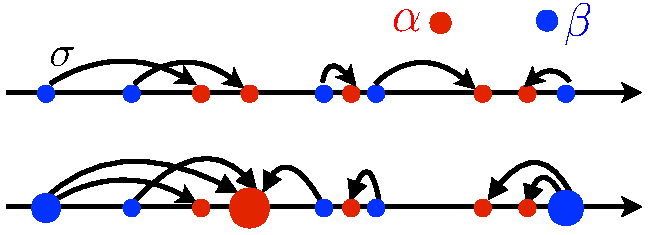
\includegraphics[width=.4\linewidth]{1d-discrete/1d-schematic}
\caption{\label{fig-1d-discrete}
1-D optimal couplings: each arrow $x_i \rightarrow y_j$ indicate a non-zero $\P_{i,j}$ in the optimal coupling.
% 
Top: empirical measures with same number of points (optimal matching).
Bottom: generic case. 
%
This corresponds to monotone rearrangements, if $x_i \leq x_{i'}$ are such that $\P_{i,j} \neq 0, \P_{i',j'} \neq 0$, then necessarily $y_j \leq y_{j'}$.
}
\end{figure}


%%%%%%%
\begin{rem}[1-D case -- Generic case]\label{rem-1d-ot-generic}
For a measure $\al$ on $\RR$, we introduce the cumulative function
\eql{\label{eq-cumul-defn}
	\foralls x \in \RR, \quad \cumul{\al}(x) \eqdef \int_{-\infty}^x \d\al, 
}
which is a function $\cumul{\al} : \RR \rightarrow [0,1]$, and its pseudo-inverse  $\cumul{\al}^{-1} : [0,1] \rightarrow \RR \cup \{-\infty\}$ \eq{
	\foralls r \in [0,1], \quad \cumul{\al}^{-1}(r) = \umin{x} \enscond{x \in \RR \cup \{-\infty\} }{ \cumul{\al}(x) \geq r }.
}
%
That function is also called the generalized quantile function of $\alpha$. For any $p \geq 1$, one has
\eql{\label{eq-wass-cumul}
	\Wass_p(\al,\be)^p = \norm{ \cumul{\al}^{-1} - \cumul{\be}^{-1} }_{L^p([0,1])}^p = \int_0^1 | \cumul{\al}^{-1}(r) - \cumul{\be}^{-1}(r) |^p \d r.
}
This means that through the map $\al \mapsto \cumul{\al}^{-1}$, the Wasserstein distance is isometric to a linear space equipped with the $L^p$ norm, or, equivalently, that the Wasserstein distance for measures on the real line is a Hilbertian metric. 
This makes the geometry of 1-D optimal transport very simple, but also very different from its geometry in higher dimensions, which is not Hilbertian as discussed in Proposition~\ref{prop-negative-definite} and more generally in~\S\ref{sec-non-embeddability}.
%
For $p=1$, one even has the simpler formula
\begin{align}\label{eq-w1-1d}
	\Wass_1(\al,\be) &= \norm{ \cumul{\al} - \cumul{\be} }_{L^1(\RR)} = 
	\int_\RR | \cumul{\al}(x) - \cumul{\be}(x) | \d x \\
	&= \int_\RR \abs{ \int_{-\infty}^x \d(\al-\be) } \d x.
\end{align}
which shows that $\Wass_1$ is a norm (see~\S\ref{sec-w1-eucl} for the generalization to arbitrary dimensions). 
%
An optimal Monge map $\T$ such that $\T_\sharp \al=\be$ is then defined by
\eql{\label{eq-OT-map-1d}
 	\T = \cumul{\be}^{-1} \circ \cumul{\al}.
}
Figure~\ref{fig-1d-ot} illustrates the computation of 1-D OT through cumulative functions. It also displays displacement interpolations, computed as detailed in~\eqref{eq-displacement-1d-cumul}, see also Remark~\ref{rem-bary-1d}. For a detailed survey of the properties of optimal transport in 1-D, we refer the reader to~\cite[Chapter 2]{SantambrogioBook}.
\end{rem}
%%%%%%%


\newcommand{\MyFigCumulMeas}[1]{\includegraphics[width=.28\linewidth]{1d-cumulative/#1}}
\newcommand{\MyFigCumulCum}[1]{\includegraphics[width=.2\linewidth]{1d-cumulative/#1}}
\begin{figure}
\centering
\begin{tabular}{@{}c@{\hspace{1mm}}c@{\hspace{1mm}}c@{}}
\MyFigCumulMeas{input-mu}&
\MyFigCumulMeas{input-nu}&
\MyFigCumulMeas{interp-bary}\\
$\mu$ & $\nu$ & ${ (t\T+(1-t)\Id)_\sharp \mu}$
\end{tabular}
%%%%
\begin{tabular}{@{}c@{\hspace{2mm}}c@{\hspace{2mm}}c@{\hspace{2mm}}c@{}}
\MyFigCumulCum{cumul}&
\MyFigCumulCum{icumul}&
\MyFigCumulCum{transports}&
\MyFigCumulCum{interp-cumul}\\
$(\cumul{\al},\cumul{\be})$ & 
$(\cumul{\al}^{-1},\cumul{\be}^{-1})$ & 
$(T,T^{-1})$ &
$(1-t)\cumul{\al}^{-1}+t\cumul{\be}^{-1}$ 
\end{tabular}
\caption{\label{fig-1d-ot}
Computation of OT and displacement interpolation between two 1-D measures, using cumulant function as detailed in~\eqref{eq-OT-map-1d}. 
}
\end{figure}

%%%%%%%
\begin{rem}[Distance between Gaussians]\label{rem-dist-gaussians}
If $\al = \Nn(\mean_\al,\cov_\al)$ and $\be = \Nn(\mean_\be,\cov_\be)$ are two Gaussians in $\RR^\dims$, then one can show that the following map
\eql{\label{eq-transport-Bures}T:x\mapsto \mean_\be + A(x-\mean_\al),}
where 
$$A=\cov_\al^{-\tfrac{1}{2}}\Big(\cov_\al^{\tfrac{1}{2}}\cov_\be\cov_\al^{\tfrac{1}{2}}\Big)^{\tfrac{1}{2}}\cov_\al^{-\tfrac{1}{2}}=\transp{A},$$
is such that $T_\sharp \rho_\al = \rho_\be$. Indeed, one simply has to notice that the change of variables formula~\eqref{eq-pfwd-density} is satisfied since
$$
\begin{aligned}\rho_\be(T(x))&=\det(2\pi\cov_\be)^{-\tfrac{1}{2}} \exp(-\dotp{T(x)-\mean_\be}{\cov_\be^{-1}(T(x)-\mean_\be)})\\
&= \det(2\pi\cov_\be)^{-\tfrac{1}{2}} \exp(-\dotp{ x-\mean_\al}{\transp{A}\cov_\be^{-1}A(x-\mean_\al)}) \\
&= \det(2\pi\cov_\be)^{-\tfrac{1}{2}} \exp(-\dotp{ x-\mean_\al}{\cov_\al^{-1}(x-\mean_\al)}),
\end{aligned}$$
and since $T$ is a linear map we have that 
$$|\det T'(x)|= \det A = \left(\frac{\det\cov_\be}{\det\cov_\al}\right)^{\tfrac{1}{2}}$$
 and we therefore recover $\rho_\al=|\det T'| \rho_\be$ meaning $T_\sharp \al = \be$. Notice now that $T$ is the gradient of the convex function $\psi:x\mapsto \tfrac{1}{2}\dotp{x-\mean_\al}{A (x-\mean_\al)} + \dotp{\mean_\be}{x}$ to conclude, using Brenier's theorem~\cite{Brenier91} (see Remark~\ref{rem-exist-mongemap}) that $T$ is optimal. Both that map $T$ and the corresponding potential $\psi$ are illustrated in Figures~\ref{fig-gaussians-2d-T} and~\ref{fig-gaussians-2d-psi}
 
 
With additional calculations involving first and second order moments of $\rho_\al$, we obtain that the transport cost of that map is
\eql{\label{eq-dist-gauss}
	\Wass_2^2( \al,\be ) = \norm{ \mean_\al - \mean_\be }^2 + \Bb(\cov_\al,\cov_\be)^2
}
where $\Bb$ is the so-called Bures' metric~\cite{bures1969extension} between positive definite matrices (see also~\cite{,forrester2016relating}),
\eql{\label{eq-bure-defn}
	\Bb(\cov_\al,\cov_\be)^2 \eqdef \tr\pa{
		\cov_\al + \cov_\be - 2 ( \cov_\al^{1/2} \cov_\be \cov_\al^{1/2} )^{1/2}
	},
}
where $\cov^{1/2}$ is the matrix square root. One can show that $\Bb$ is a distance on covariance matrices, and that $\Bb^2$ is convex with respect to both its arguments. 
In the case where $\cov_\al = \diag(r_i)_i$ and $\cov_\be = \diag(s_i)_i$ are diagonals, the Bures metric is the Hellinger distance
\eq{
	\Bb(\cov_\al,\cov_\be) = \norm{ \sqrt{r}-\sqrt{s} }_2.
}
For 1-D Gaussians, $\Wass_2$ is thus the Euclidean distance on the 2-D plane $(\mean,\sqrt{\cov})$, as illustrated in Figure~\ref{fig-1d-gaussian}. 
%
For a detailed treatment of the Wasserstein geometry of Gaussian distributions, we refer to~\cite{takatsu2011wasserstein}.
\end{rem}
%%%%%%



\begin{figure}
\centering
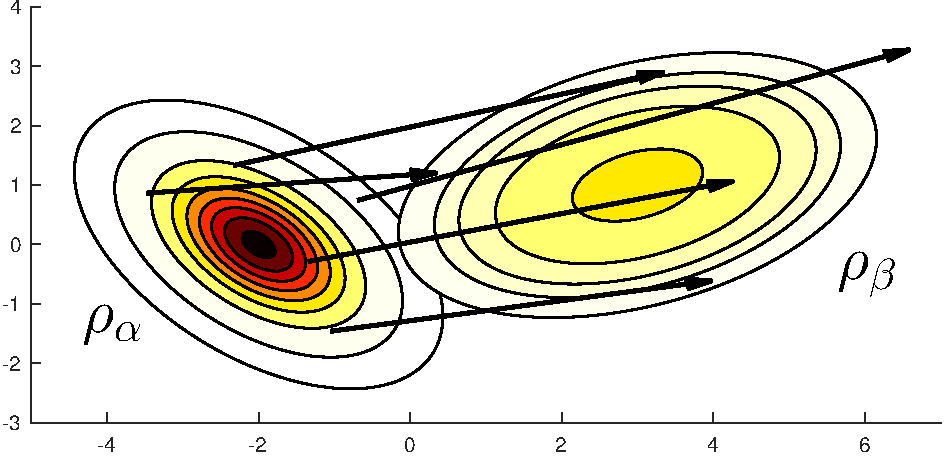
\includegraphics[width=.4\linewidth]{gaussians-2d/gaussians1.pdf}
\caption{\label{fig-gaussians-2d-T} Two Gaussians $\rho_\al$ and $\rho_\be$, represented using the contour plots of their densities, with respective mean and variance matrices $\mean_\al=(-2,0),\cov_\al=\frac{1}{2}\left(1 -\tfrac{1}{2};-\tfrac{1}{2}  1\right)$ and $\mean_\be=(3,1), \cov_\be=\left(2, \tfrac{1}{2}; \tfrac{1}{2}, 1\right)$. The arrows originate at random points $x$ taken on the plane and end at the corresponding mappings of those points $T(x)=\mean_\be + A(x-\mean_\al)$.}
\end{figure}



\begin{figure}
\centering
\begin{tabular}{@{}c@{\hspace{15mm}}c@{}}
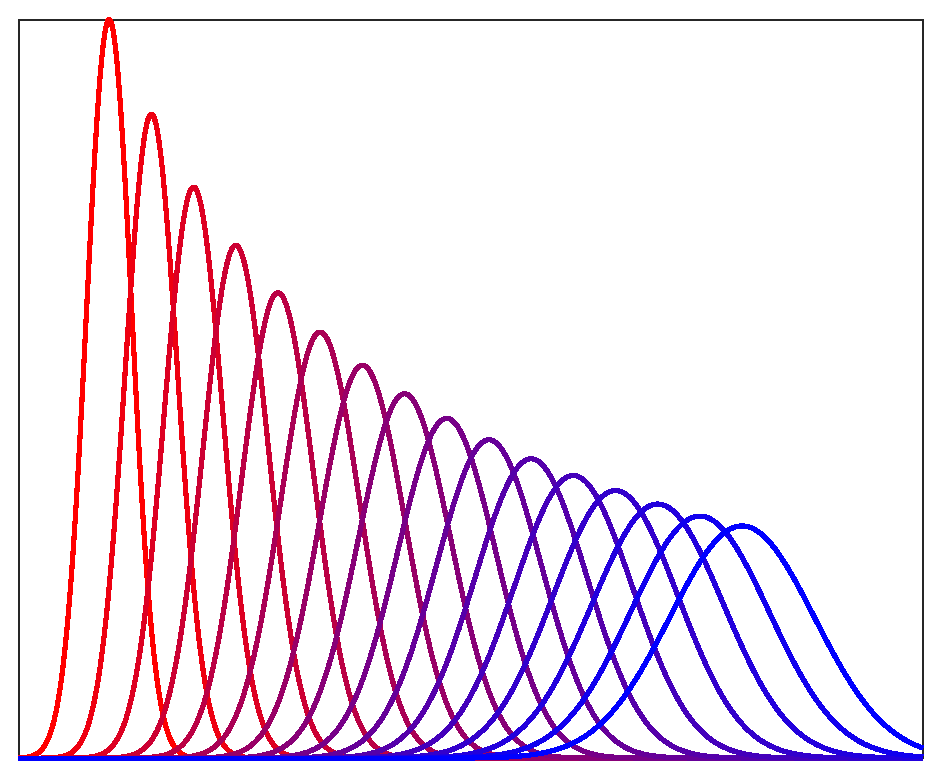
\includegraphics[width=.25\linewidth]{gaussian-1d/interp-density}&
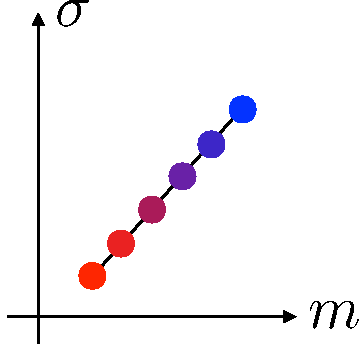
\includegraphics[width=.2\linewidth]{gaussian-1d/gaussian-param}
\end{tabular}
\caption{\label{fig-1d-gaussian}
Computation of displacement interpolation between two 1-D Gaussians. 
%
Denoting $\Gg_{m,\si}(x) \eqdef \frac{1}{\sqrt{2\pi}s}e^{-\frac{(x-m)^2}{2s^2}}$ the Gaussian density, it thus shows 
the interpolation $\Gg_{(1-t)m_0+t m_1,(1-t)\si_0+t \si_1}$.
}
\end{figure}



%%%%%%%%%%%%%%%%%%%%%%%%%%%%%%%%%%%%%%%%%%%%%%%%%%%%%%%%%%%%%%%%%%%%%%%%%%%%%%%%%%%%%%%%%%
%\paragraph{$W_1$ theory} 

%Lipschitz functions, min-cost flow.


%%% HERE %%%

%%%%%%%%%%%%%%%%%%%%%%%%%%%%%%%%%%%%%%%%%%%%%%%%%%%%%%%%%%%%%%%%%%%%%%%%%%%%%%%%%%%%%%%%%%
%%%%%%%%%%%%%%%%%%%%%%%%%%%%%%%%%%%%%%%%%%%%%%%%%%%%%%%%%%%%%%%%%%%%%%%%%%%%%%%%%%%%%%%%%%
%%%%%%%%%%%%%%%%%%%%%%%%%%%%%%%%%%%%%%%%%%%%%%%%%%%%%%%%%%%%%%%%%%%%%%%%%%%%%%%%%%%%%%%%%%
\section{Sinkhorn}
\label{sec-sinkhorn}

This section introduces a family of numerical scheme to approximate solutions to Kantorovich formulation of optimal transport and its many generalizations. It operates by adding an entropic regularization penalty to the original problem. This regularization has several important advantages, but a few stand out particularly: The minimization of the regularized problen can be solved using a simple alternate minimization scheme; that scheme translates into iterations that are simple matrix products, making them particularly suited to execution of GPU; the resulting approximate distance is smooth with respect to input histogram weights and positions of the Diracs.

%%%%%%%%%%%%%%%%%%%%%%%%%%%%%%%%%%%%%%%%%%%
\paragraph{Entropic Regularization.}

The discrete entropy of a coupling matrix is defined as
\eql{\label{eq-discr-entropy}
	\HD(\P) \eqdef -\sum_{i,j} \P_{i,j} (\log(\P_{i,j})-1), 
}
with an analogous definition for vectors, with the convention that $\HD(\a) = -\infty$ if one of the entries $\a_j$ is 0 or negative. The function $\HD$ is 1-strongly concave, because its hessian is $\partial^2 \HD(P)=-\diag(1/\P_{i,j})$ and $\P_{i,j} \leq 1$. The idea of the entropic regularization of optimal transport is to use $-\HD$ as a regularizing function to obtain approximate solutions to the original transport problem~\eqref{eq-mk-discr}:
\eql{\label{eq-regularized-discr}
	\MKD_\C^\epsilon(\a,\b) \eqdef 
	\umin{\P \in \CouplingsD(\a,\b)}
		\dotp{\P}{\C} - \epsilon \HD(\P). 
} 
Since the objective is a $\epsilon$-strongly convex function, problem~\ref{eq-regularized-discr} has a unique optimal solution. The idea to regularize the optimal transport problem by an entropic term can be traced back to modeling ideas in transportation theory~\cite{wilson1969use}: Actual traffic patterns in a network do not agree with those predicted by the solution of the optimal transport problem. Indeed, the former are more diffuse than the latter, which tend to rely on a few routes as a result of the sparsity of optimal couplings to the solution of~\ref{eq-mk-discr}. To balance for that, researchers in transportation proposed a model, called the ``gravity'' model~\cite{erlander1980optimal}, that is able to form a more ``blurred'' traffic prediction. 

Figure~\ref{fig-impact-eps} illustrates the effect of the entropy to regularize a linear program over the simples $\simplex_3$ (which can thus be visualized as a triangle in 2-D). Note how the entropy pushes the original LP solution away from the boundary of the triangle. The optimal $\P_\epsilon$ progressively moves toward an ``entropic center'' of the triangle. This is further detailed in the proposition below. The convergence of the solution of that regularized problem towards an optimal solution of the original linear program has been studied by~\cite{CominettiAsympt}.


\begin{figure}
\centering
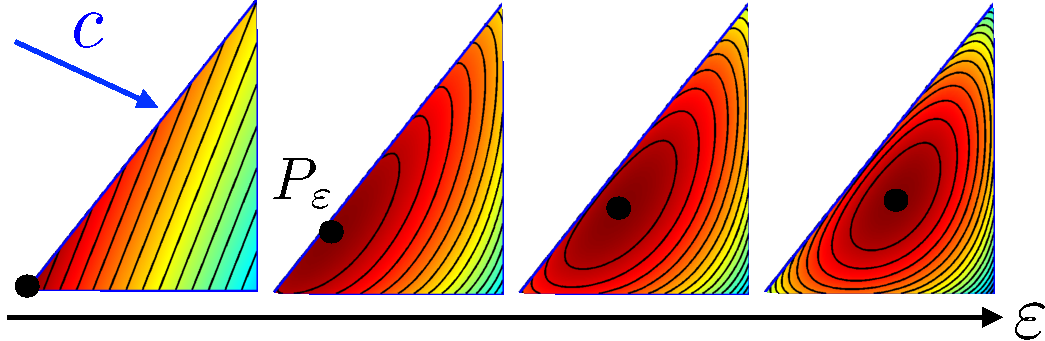
\includegraphics[width=.5\linewidth]{entropic/simplex}
\caption{\label{fig-impact-eps}
Impact of $\epsilon$ on the optimization of a linear function on the simplex, solving $\P_\epsilon = \argmin_{\P \in \simplex_3} \dotp{\C}{\P}-\epsilon\HD(\P)$ for a varying $\epsilon$. 
}
\end{figure}


\begin{prop}[Convergence with $\epsilon$]\label{prop-convergence-eps}
The unique solution $\P_\epsilon$ of~\eqref{eq-regularized-discr} converges to the optimal solution with maximal entropy within the set of all optimal solutions of the Kantorovich problem, namely
\eql{\label{eq-entropy-conv-1}
	\P_\epsilon \overset{\epsilon \rightarrow 0}{\longrightarrow}
	\uargmin{\P} \enscond{ -\HD(\P) }{
		\P \in \CouplingsD(\a,\b), \dotp{\P}{\C} = \MKD_\C(\a,\b)
	}
}
so that in particular
\eq{
	\MKD_\C^\epsilon(\a,\b) \overset{\epsilon \rightarrow 0}{\longrightarrow} \MKD_\C(\a,\b).
}
One has
\eql{\label{eq-entropy-conv-2}
	\P_\epsilon \overset{\epsilon \rightarrow \infty}{\longrightarrow}
	\a \transp{\b} = (\a_i \b_j)_{i,j}.
}
\end{prop}

\begin{proof}
	 We consider a sequence $(\epsilon_\ell)_\ell$ such that $\epsilon_\ell \rightarrow 0$ and $\epsilon_\ell > 0$.	
 	We denote $\P_\ell$ the solution of~\eqref{eq-regularized-discr} for $\epsilon=\epsilon_\ell$. 
	%
	Since $\CouplingsD(\a,\b)$ is bounded, we can extract a sequence (that we do not relabel for sake of simplicity) such that $\P_\ell \rightarrow \P^\star$. Since $\CouplingsD(\a,\b)$ is closed, $\P^\star \in \CouplingsD(\a,\b)$. We consider any $\P$ such that $\dotp{\C}{\P} = \MKD_\C(\a,\b)$. By optimality of $\P$ and $\P_\ell$ for their respective optimization problems (for $\epsilon=0$ and $\epsilon=\epsilon_\ell$), one has
 	\eql{\label{eq-proof-gamma-conv}
 		0 \leq \dotp{\C}{\P_\ell} - \dotp{\C}{\P} \leq \epsilon_\ell ( \HD(\P_\ell)-\HD(\P) ).
 	}
 	Since $\HD$ is continuous, taking the limit $\ell \rightarrow +\infty$ in this expression shows that 
 	$\dotp{\C}{\P^\star} = \dotp{\C}{\P}$ so that $\P^\star$ is a feasible point of~\eqref{eq-entropy-conv-1}. Furthermore, dividing by $\epsilon_\ell$ in~\eqref{eq-proof-gamma-conv} and taking the limit shows that 
 	$\HD(\P) \leq \HD(\P^\star)$, which shows that $\P^\star$ is a solution of~\eqref{eq-entropy-conv-1}. Since the solution $\P_0^\star$ to this program is unique by strict convexity of $-\HD$, one has $\P^\star = \P_0^\star$, and the whole sequence is converging. 
\end{proof}

Formula~\eqref{eq-entropy-conv-1} states that for low regularization, the solution converges to the maximum entropy optimal transport coupling.
%
In sharp contrast,~\eqref{eq-entropy-conv-2} shows that for large regularization, the solution converges to the coupling with maximal entropy between two prescribed marginals $\a,\b$, namely the joint probability between two independent random variables with prescribed distributions.
%
A refined analysis of this convergence is performed in~\cite{CominettiAsympt}, including a first order expansion in $\epsilon$ (resp. $1/\epsilon$) near $\epsilon=0$ (resp $\epsilon=+\infty$).
%
Figure~\ref{fig-entropic} shows visually the effect of these two convergence. A key insight is that, as $\epsilon$ increases, the optimal coupling becomes less and less sparse (in the sense of having entries larger than a prescribed thresholds), which in turn as the effect of both accelerating computational algorithms (as we study in~\S\ref{sec-sinkhorn}) but also leading to faster statistical convergence (as exposed in~\S\ref{sec-entropy-ot-mmd}). 

\begin{figure}
\centering
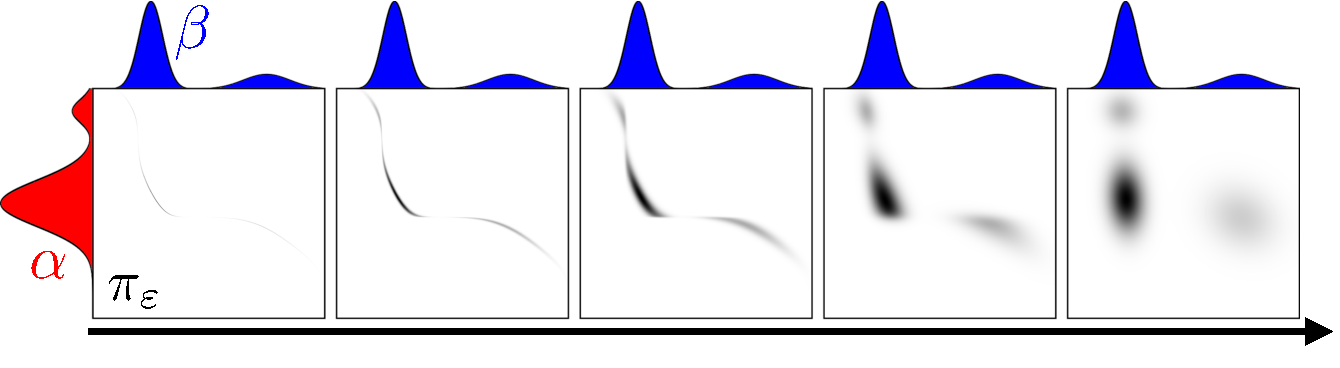
\includegraphics[width=.48\linewidth]{entropic/densities}
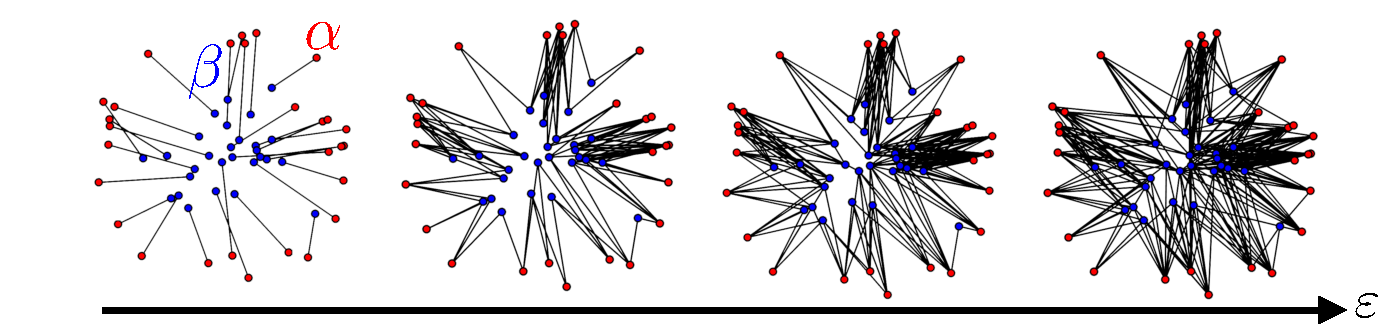
\includegraphics[width=.48\linewidth]{entropic/matching-2d}
\caption{\label{fig-entropic}
Impact of $\epsilon$ on coupling between densities and discrete distributions, illustrating Proposition~\ref{prop-convergence-eps}.
%
Left: between two 1-D densities. Right: between two 2-D discrete empirical densities with same number $n=m$ of points (only entries of the optimal $(\P_{i,j})_{i,j}$ above a small threshold are displayed as segments between $x_i$ and $y_j$).
}
\end{figure}

Defining the Kullback-Leibler divergence between couplings as
\eql{\label{eq-kl-defn}
	\KLD(\P|\K) \eqdef \sum_{i,j}  \P_{i,j} \log\pa{\frac{\P_{i,j}}{\K_{i,j}}} - \P_{i,j} + \K_{i,j},
}
the unique solution $\P_\epsilon$ of~\eqref{eq-regularized-discr} is a projection onto $\CouplingsD(\a,\b)$ of the Gibbs kernel associated to the cost matrix $\C$ as
\eq{
	\K_{i,j} \eqdef e^{-\frac{\C_{i,j}}{\epsilon}}
}
Indeed one has that using the definition above
\eql{\label{eq-kl-proj}
	\P_\epsilon = \Proj_{\CouplingsD(\a,\b)}^\KLD(\K) \eqdef \uargmin{\P \in \CouplingsD(\a,\b)} \KLD(\P|\K).
}



%%%%%
\begin{rem}[General formulation]
One can consider arbitrary measures by replacing the discrete entropy by the relative entropy with respect to the product measure $\d\al\otimes\d\be(x,y) \eqdef \d\al(x)\d\be(y)$, and propose a regularized counterpart to~\eqref{eq-mk-generic} using
\eql{\label{eq-entropic-generic}
	\MK_\c^\epsilon(\al,\be) \eqdef 
	\umin{\pi \in \Couplings(\al,\be)}
		\int_{X \times Y} c(x,y) \d\pi(x,y) + \epsilon \KL(\pi|\al\otimes\be)
}
where the relative entropy is a generalization of the discrete Kullback-Leibler divergence~\eqref{eq-kl-defn}
\eql{\label{eq-defn-rel-entropy}
\begin{aligned}	 \KL(\pi|\xi) \eqdef \int_{\X \times \Y} \log\Big( \frac{\d \pi}{\d\xi}(x,y) \Big) \d\pi(x,y)
	  +\\ \int_{\X \times \Y} (\d\xi(x,y)-\d\pi(x,y)), 
	  \end{aligned}
}
and by convention $\KL(\pi|\xi)=+\infty$ if $\pi$ does not have a density $\frac{\d \pi}{\d\xi}$ with respect to $\xi$. 
%
It is important to realize that the reference measure $\al\otimes\be$ chosen in~\eqref{eq-entropic-generic} to define the entropic regularizing term $\KL(\cdot|\al\otimes\be)$ plays no specific role, only its support matters.

Formula~\eqref{eq-entropic-generic} can be re-factored as a projection problem
\eql{\label{eq-entropic-generic-proj}
	\umin{\pi \in \Couplings(\al,\be)} \KL(\pi|\Kk)
}
where $\Kk$ is the Gibbs distributions $\d\Kk(x,y) \eqdef e^{-\frac{c(x,y)}{\epsilon}} \d\mu(x)\d\nu(y)$.
%
This problem is often referred to as the ``static Schr\"odinger problem''~\cite{LeonardSchroedinger,RuschendorfThomsen}, since it was initially considered by Schr\"odinger in statistical physics~\cite{Schroedinger31}. 
%
As $\epsilon \rightarrow 0$, the unique solution to~\eqref{eq-entropic-generic-proj} converges to the maximum entropy solution to~\eqref{eq-mk-generic}, see~\cite{leonard2012schrodinger,2017-carlier-SIMA}.
%
~\S\ref{sec-entropic-dynamic} details an alternate ``dynamic'' formulation of the Schr\"odinger problem over the space of paths connecting the points of two measures.
\end{rem}
%%%%%




%%%%%%%%%%%%%%%%%%%%%%%%%%%%%%%%%%%%%%%%%%%
\paragraph{Sinkhorn's Algorithm}

The following proposition shows that the solution of~\eqref{eq-regularized-discr} has a specific form, which can be parameterized using $n+m$ variables. That parameterization is therefore essentially dual, in the sense that a coupling $\P$ in $\CouplingsD(\a,\b)$ has $nm$ variables but $n+m$ constraints.

\begin{prop}\label{prop-regularized-primal}
The solution to~\eqref{eq-regularized-discr} is unique and has the form
\eql{\label{eq-scaling-form}
	\foralls (i,j) \in \range{n} \times \range{m}, \quad \P_{i,j} = \uD_i \K_{i,j} \vD_j
}
for two (unknown) scaling variable $(\uD,\vD) \in \RR_+^n \times \RR_+^m$. 
\end{prop} 

\begin{proof} 
Introducing two dual variables $\fD\in\RR^n,\gD\in\RR^m$ for each marginal constraint, the Lagrangian of~\eqref{eq-regularized-discr} reads
\eq{\label{eq-sinkhorn-lagrangian}
	\Lag(\P,\fD,\gD)= \dotp{\P}{\C} - \epsilon \HD(\P) - \dotp{\fD}{\P\ones_m-\a}-\dotp{\gD}{\transp{\P}\ones_n-\b}.
}
Considering first order conditions, we have
$$
	\frac{\partial\Lag(\P,\fD,\gD)}{\partial \P_{i,j}}= \C_{i,j} - \epsilon \log(\P_{i,j}) - \fD_i -\gD_j.
$$
which results, for an optimal $\P$ coupling to the regularized problem, in the expression $\P_{i,j}=e^{\fD_i/\varepsilon}e^{-\C_{i,j}/\varepsilon}e^{\gD_j/\varepsilon}$ which can be rewritten in the form provided in the proposition using non-negative vectors $\uD$ and $\vD$.
\end{proof} 

The factorization of the optimal solution exhibited in Equation~\eqref{eq-scaling-form} can be conveniently rewritten in matrix form as $\P=\diag(\uD)\K\diag(\vD)$.
%
$\uD,\vD$ must therefore satisfy the following non-linear equations which correspond to the mass conservation constraints inherent to $\CouplingsD(\a,\b)$,
\eql{\label{eq-dualsinkhorn-constraints}
	\diag(\uD)\K\diag(\vD)\ones_m=\a,
	\qandq
	\diag(\vD)\K^\top \diag(\uD)\ones_n=\b,
}
These two equations can be further simplified, since $\diag(\vD)\ones_m$ is simply $\vD$, and the multiplication of $\diag(\uD)$ times $\K \vD$ is 
\eql{\label{eq-dualsinkhorn-constraints2}
	\uD \odot (\K \vD) = \a
	\qandq
	\vD \odot (\transp{\K}\uD) = \b
}
where $\odot$ corresponds to entry-wise multiplication of vectors. That problem is known in the numerical analysis community as the matrix scaling problem (see~\cite{nemirovski1999complexity} and references therein).
%
An intuitive way to try to solve these equations is to solve them iteratively, by modifying first $\uD$ so that it satisfies the left-hand side of Equation~\eqref{eq-dualsinkhorn-constraints2} and then $\vD$ to satisfy its right-hand side. These two updates define Sinkhorn's algorithm:
\eql{\label{eq-sinkhorn}	
	\itt{\uD} \eqdef \frac{\a}{\K \it{\vD}}
	\qandq
	\itt{\vD} \eqdef \frac{\b}{\transp{\K}\itt{\uD}},
}
initialized with an arbitrary positive vector $\init{\vD} = \ones_m$. The division operator used above between two vectors is to be understood entry-wise. Note that a different initialization will likely lead to a different solution for $\uD,\vD$, since $\uD,\vD$ are only defined up to a multiplicative constant (if $\uD,\vD$ satisfy \eqref{eq-dualsinkhorn-constraints} then so do $\lambda\uD,\vD/\lambda$ for any $\lambda>0$).
%
It turns out however that these iterations converge (see Remark~\ref{rem-iterative-projection} for a justification using iterative projections, and Remark~\ref{rem-global-conv-sinkh} for a strict contraction result) and all result in the same optimal coupling $\diag(\uD)\K\diag(\vD)$. 
%
Figure~\ref{fig-sinkhorn-convergence}, top row, shows the evolution of the coupling $\diag(\it{\UD})\K\diag(\it{\VD})$ computed by Sinkhorn iterations. It  evolves from the Gibbs kernel $\K$ towards the optimal coupling solving~\eqref{eq-regularized-discr} by progressively shifting the mass away from the diagonal.


\begin{figure}
\centering
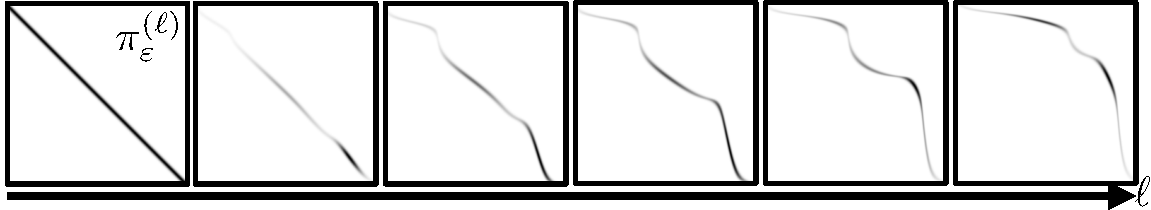
\includegraphics[width=.7\linewidth]{entropic/sinkhorn-convergence}
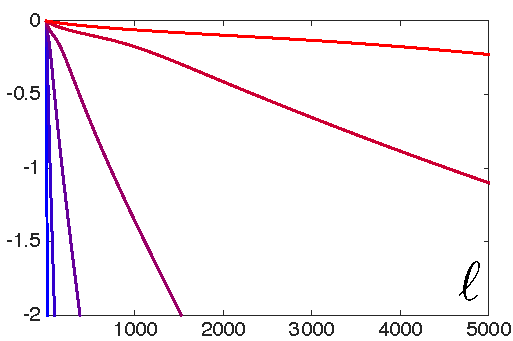
\includegraphics[width=.28\linewidth]{entropic/sinkhorn-rates}
\caption{\label{fig-sinkhorn-convergence}
Left: evolution of the coupling $\pi_\epsilon^\ell=\diag(\it{\UD})\K\diag(\it{\VD})$ computed at iteration $\ell$ of Sinkhorn's iterations, for 1-D densities.
Right: impact of $\epsilon$ the convergence rate of Sinkhorn, as measured in term of marginal constraint violation $\log( \norm{\pi_\epsilon^\ell \ones_m - \b}_1 )$.
}
\end{figure}


%%%%%%%
\begin{rem}[Relation with iterative projections]\label{rem-iterative-projection}
Denoting 
\eq{
	\Cc^1_\a \eqdef \enscond{\P}{\P\ones_m=\a}
	\qandq
	\Cc^2_\b \eqdef \enscond{\P}{\transp{\P}\ones_m=\b}
}
the rows and columns constraints, one has $\CouplingsD(\a,\b) = \Cc^1_\a \cap \Cc^2_\b$. One can use Bregman iterative projections~\cite{bregman1967relaxation}
\eql{\label{eq-kl-sinkh-proj}
	\itt{\P} \eqdef \Proj_{\Cc^1_\a}^{\KLD}(\it{\P})
	\qandq
	\ittt{\P} \eqdef \Proj_{\Cc^2_\b}^{\KLD}(\itt{\P}).
}
Since the sets $\Cc^1_\a$ and $\Cc^2_\b$ are affine, these iterations are known to converge to the solution of~\eqref{eq-kl-proj}, see~\cite{bregman1967relaxation}. These iterate are equivalent to Sinkhorn iterations~\eqref{eq-sinkhorn} since defining 
\eq{\label{eq-sink-matrix}\P^{(2\ell)} \eqdef \diag(\it{\uD}) \K \diag(\it{\vD}),}
one has
\begin{align*}
	\P^{(2\ell+1)} &\eqdef \diag(\itt{\uD}) \K \diag(\it{\vD}) \\
	\qandq
	\P^{(2\ell+2)} &\eqdef \diag(\itt{\uD}) \K \diag(\itt{\vD})
\end{align*}
In practice however one should prefer using~\eqref{eq-sinkhorn} which only requires manipulating scaling vectors and multiplication against a Gibbs kernel, which can often be accelerated (see below Remarks~\ref{rem-separable} and~\ref{rem-geod-heat}). 
\end{rem}
%%%%%%%



%%%%%%%%%%
\begin{rem}[Hilbert metric]
As initially explained by~\cite{franklin1989scaling}, the global convergence analysis of Sinkhorn is greatly simplified using Hilbert projective metric on $\RR_{+,*}^n$ (positive vectors), defined as
\eq{
	\foralls (\uD,\uD') \in (\RR_{+,*}^n)^2, \quad
	\Hilbert(\uD,\uD') \eqdef \log \umax{i,i'} \frac{ \uD_i \uD_{i'}' }{ \uD_{i'} \uD_{i}'  }.
}
This can be shows to be a distance on the projective cone $\RR_{+,*}^n/\sim$, where $\uD \sim \uD'$ means that $\exists s>0, \uD=s\uD'$ (the vector are equal up to rescaling, hence the naming ``projective'').  
%
This means that $\Hilbert$ satisfies the triangular inequality and $\Hilbert(\uD,\uD')=0$ if and only if $\uD \sim \uD'$. 
%
This is a projective version of Hilbert's original distance on bounded open convex sets~\cite{hilbert1895gerade}.
%
The projective cone $\RR_{+,*}^n/\sim$ is a complete metric space for this distance. 
%
It was introduced independently by~\cite{birkhoff1957extensions} and~\cite{samelson1957perron} to provide a quantitative proof of Perron-Frobenius theorem, which, as explained in Remark~\ref{rem-local-conv} is linked to a local linearization of Sinkhorn's iterates. They proved the following fundamental theorem, which shows that a positive matrix is a strict contraction on the cone of positive vectors.

\begin{thm}\label{thm-birkoff}
	Let $\K \in \RR_{+,*}^{n \times m}$, then for $(\vD,\vD') \in (\RR_{+,*}^m)^2$
	\eq{
		\Hilbert(\K \vD,\K \vD') \leq \la(\K) \Hilbert(\vD,\vD')
		\text{ where }
		\choice{
			\la(\K) \eqdef \frac{ \sqrt{\eta(\K)}-1 }{ \sqrt{\eta(\K)}+1 } < 1 \\
			\eta(\K) \eqdef \umax{i,j,k,\ell} \frac{ \K_{i,k} \K_{j,\ell} }{ \K_{j,k} \K_{i,\ell} }.
		}
	}
\end{thm}
\end{rem}
%%%%%%%%%%

%%%%%%%%%%
\begin{rem}[Global convergence]\label{rem-global-conv-sinkh}
The following theorem, proved by~\cite{franklin1989scaling}, makes use of this Theorem~\ref{thm-birkoff} to show the linear convergence of Sinkhorn's iterations.

\begin{thm}
	One has $(\it{\uD},\it{\vD}) \rightarrow (\uD^\star,\vD^\star)$ and
	\eql{\label{eq-convlin-sinkh}
		\Hilbert(\it{\uD}, \uD^\star) = O(\la(\K)^{2\ell}), \quad
		\Hilbert(\it{\vD}, \vD^\star) = O(\la(\K)^{2\ell}).
	}
	One also has
	\eql{\label{eq-convsinkh-control}
		\begin{split}
		\Hilbert(\it{\uD}, \uD^\star) &\leq \frac{\Hilbert( \it{\P}\ones_m,\a )}{1-\la(\K)} \\
		\Hilbert(\it{\vD}, \vD^\star) &\leq \frac{\Hilbert( \P^{(\ell),\top} \ones_n,\b )}{1-\la(\K)}
		\end{split}
	}
	where we denoted $\it{\P} \eqdef \diag(\it{\uD}) \K \diag(\it{\vD})$. Lastly, one has
	\eql{\label{eq-convlin-sinkh-prim}
		\|\log(\it{\P}) - \log(\P^\star)\|_\infty \leq \Hilbert(\it{\uD}, \uD^\star) + \Hilbert(\it{\vD}, \vD^\star)
	}
	where $\P^\star$ is the unique solution of~\eqref{eq-regularized-discr}. 
\end{thm}

\begin{proof}
	One notice that for any $(\vD,\vD') \in (\RR_{+,*}^m)^2$, one has 
	\eq{	
		\Hilbert(\vD,\vD') = \Hilbert(\vD/\vD',\ones_m) = \Hilbert(\ones_m/\vD,\ones_m/\vD').
	}
	This shows that
	\begin{align*}
		\Hilbert(\itt{\uD},\uD^\star) &= \Hilbert\pa{ \frac{\a}{\K \it{\vD}}, \frac{\a}{\K \vD^\star} } \\
		&= \Hilbert( \K \it{\vD}, \K \vD^\star ) \leq \la(\K) \Hilbert( \it{\vD}, \vD^\star ).
	\end{align*}
	where we used Theorem~\ref{thm-birkoff}. This shows~\eqref{eq-convlin-sinkh}.  One also has, using the triangular inequality
	\begin{align*}
		\Hilbert(\it{\uD},\uD^\star) &\leq \Hilbert(\itt{\uD},\it{\uD}) + \Hilbert(\itt{\uD},\uD^\star) \\
		&\leq \Hilbert\pa{ \frac{\a}{\K \it{\vD}},\it{\uD} } + \la(\K) \Hilbert(\it{\uD},\uD^\star) \\
		&= \Hilbert\pa{ \a,\it{\uD} \odot  ( \K \it{\vD} ) } + \la(\K) \Hilbert(\it{\uD},\uD^\star), 
	\end{align*}
	which gives the first part of~\eqref{eq-convsinkh-control} since 
	$\it{\uD} \odot  ( \K \it{\vD} ) = \it{\P}\ones_m$ (the second one being similar).
	%
	The proof of~\eqref{eq-convlin-sinkh-prim} follows from~\cite[Lemma 3]{franklin1989scaling}
\end{proof}
 
The bound~\eqref{eq-convsinkh-control} shows that some error measures on the marginal constraints violation, for instance $\| \it{\P} \ones_m - \a \|_1$ and $\|\transp{\it{\P}} \ones_n - \b \|_1$, are useful stopping criteria to monitor the convergence. 

Figure~\ref{fig-sinkhorn-convergence}, bottom row, highlights this linear rate on the constraint violation, and shows how this rate degrades as $\epsilon\rightarrow 0$. 
%
These results are proved in~\cite{franklin1989scaling} and are tightly connected to nonlinear Perron-Frobenius Theory~\cite{lemmens2012nonlinear}. Perron-Frobenius theory corresponds to the linearization of the iterations, see~\eqref{eq-linearized-sinkh}. This convergence analysis is extended in~\cite{linial1998deterministic}, who shows that each iteration of Sinkhorn increases the permanent of the scaled coupling matrix. 
\end{rem}
%%%%%%%%%%


%%%%%%%%%%%%%%%%%%%%%%%%%%%%%%%%%%%%%%%%%%%%
\paragraph{Regularized Dual and Log-domain Computations}

The following proposition details the dual problem associated to~\eqref{eq-regularized-discr}.

\begin{prop}
One has
\eql{\label{eq-dual-formulation}
	\MKD_\C^\epsilon(\a,\b) = \umax{\fD \in \RR^n,\gD \in \RR^m}
		 \dotp{\fD}{\a} + \dotp{\gD}{\b} 
		% - \epsilon\sum_{i,j} e^{ \frac{\fD_i+\gD_j-\C_{i,j}}{\epsilon} }.
		- \epsilon \dotp{e^{\fD/\epsilon} }{ \K e^{\gD/\epsilon}}.
} 
%
The optimal $(\fD,\gD)$ are linked to scalings $(\uD,\vD)$ appearing in~\eqref{eq-scaling-form} through 
\eql{\label{eq-entropy-pd}
	(\uD,\vD)=(e^{\fD/\epsilon},e^{\gD/\epsilon}).
}
\end{prop}

\begin{proof}
We start from the end of the proof of Proposition~\ref{prop-regularized-primal}, which links the optimal primal solution $\P$ and dual multipliers $\fD$ and $\gD$ for the marginal constraints as $\P_{i,j}=e^{\fD_i/\varepsilon}e^{-\C_{i,j}/\varepsilon}e^{\gD_j/\varepsilon}$. Substituting in the Lagrangian $\Lag(\P,\fD,\gD)$ of Equation~\eqref{eq-sinkhorn-lagrangian} the optimal $\P$ as a function of $\fD$ and $\gD$, we obtain that the Lagrange dual function equals
\eql{\label{eq-lagrange-dual-naive}
	\fD,\gD \mapsto \dotp{e^{\fD/\epsilon}}{\left(\K\odot \C\right)e^{\gD/\epsilon}} - \epsilon \HD(\diag(e^{\fD/\epsilon}) \K \diag(e^{\gD/\epsilon})).
}
The entropy of $\P$ scaled by $\epsilon$, namely $\epsilon \dotp{\P}{\log \P - \ones_{n\times m}}$ can be stated explicitly as a function of $\fD,\gD, \C$
\begin{align*}
&\dotp{\diag(e^{\fD/\epsilon}) \K \diag(e^{\gD/\epsilon})}{\fD\transp{\ones_m}+\ones_n\transp{\gD}-\C-\epsilon\ones_{n\times m}}\\
&= -\dotp{e^{\fD/\epsilon}}{\left(\K\odot \C\right)e^{\gD/\epsilon}} + \dotp{\fD}{\a}+ \dotp{\gD}{\b}-\epsilon \dotp{e^{\fD/\epsilon}}{\K e^{\gD/\epsilon}}
\end{align*}
therefore, the first term in~\eqref{eq-lagrange-dual-naive} cancels out with the first term in the entropy above. The remaining times are those displayed in~\eqref{eq-dual-formulation}.
\end{proof}


%%%%%%%%%%
\begin{rem}{Dual for generic measures}
For generic (non-necessarily discrete) input measures $(\al,\be)$, the dual problem~\eqref{eq-dual-formulation} reads
\begin{align*}
	\usup{\f,\g \in \Cc(\X)\times\Cc(\Y)} \int_\X \f(x)\d\al(x) + \int_\Y \g(x)\d\be(x) 
		 - \epsilon \int_{\X\times\Y} e^{ \frac{-c(x,y)+f(x)+g(y)}{\epsilon} } \d\al(x)\d\be(y)
\end{align*}
This corresponds to a smoothing of the constraint $\Potentials(\c)$ appearing in the original problem~\eqref{eq-dual-generic}, which is retrieved in the limit $\epsilon \rightarrow 0$.
%
Proving existence (\emph{i.e.} the sup is actually a max) of these Kantorovich potentials $(\f,\g)$ in the case of entropic transport is less easy than for classical OT (because one cannot use $c$-transform and potentials are not automatically Lipschitz). Proof of existence can be done using the convergence of Sinkhorn iterations, see~\cite{2016-chizat-sinkhorn} for more details. 
\end{rem}
%%%%%%%%%%


%%%%%%%%%%
\begin{rem}[Sinkhorn as a Block Coordinate Ascent on the Dual Problem]\label{rem-sinkh-block}
A simple approach to solve the unconstrained maximization problem~\eqref{eq-dual-formulation} is to use an exact \emph{block coordinate ascent} strategy, namely to update alternatively $\fD$ and $\gD$ to cancel their gradients with respect to the objective of \eqref{eq-dual-formulation}. Indeed, one can easily notice that, writing $Q(\fD,\gD)$ for the objective of~\eqref{eq-dual-formulation} that 
\begin{align}
	\label{eq-dualupadate-sinkh-1}\nabla|_\fD\, Q(\fD,\gD) &=  \a - e^{\fD/\epsilon}\odot \left(\K e^{\gD/\epsilon}\right),\\
	\label{eq-dualupadate-sinkh-2}\nabla|_\gD\, Q(\fD,\gD) &=  \b - e^{\gD/\epsilon}\odot \left(\K^T e^{\fD/\epsilon}\right).
\end{align}
Block coordinate ascent can therefore be implemented in a closed form by applying successively the following updates, starting from any arbitrary $\init{\gD}$, for $l\geq 0$,
\begin{align}
	\label{eq-slse-sinkh-1}\itt{\fD} &= \epsilon \log \a -\epsilon\log\left(\K e^{\it{\gD}/\epsilon}\right), \\
	\label{eq-slse-sinkh-2}\itt{\gD} &= \epsilon \log \b- \epsilon\log\left(\transp{\K} e^{\itt{\fD}/\epsilon}\right).
\end{align}
Such iterations are mathematically equivalent to the Sinkhorn iterations~\eqref{eq-sinkhorn} when considering the primal-dual relations highlighted in~\eqref{eq-entropy-pd}. Indeed, we recover that at any iteration
\eq{
	(\it{\fD},\it{\gD}) = \epsilon ( \log(\it{\uD}), \log(\it{\vD}) ). 
}
\end{rem}
%%%%%%%%%%

%%%%%%%%%%
\begin{rem}[Soft-min rewriting]
Iterations~\eqref{eq-slse-sinkh-1} and~\eqref{eq-slse-sinkh-2} can be given an alternative interpretation, using the following notation. Given a vector $\z$ of real numbers we write $\smine\z$ for the \emph{soft-minimum} of its coordinates, namely
$$
\smine\z= -\epsilon \log \sum_i e^{-\z_i/\epsilon}.
$$
Note that $\smine(\z)$ converges to $\min\,\z$ for any vector $\z$ as $\epsilon\rightarrow 0$. Indeed, $\smine$ can be interpreted as a differentiable approximation of the $\min$ function. Using these notations, Equations~\eqref{eq-slse-sinkh-1} and~\eqref{eq-slse-sinkh-2} can be rewritten
\begin{align}
\label{eq-slse-smin-1}(\itt{\fD})_i &= \smine\, (\C_{ij}-\it{\gD}_j)_j + \epsilon \log \a_i, \\
\label{eq-slse-smin-2}(\itt{\gD})_j &= \smine\, (\C_{ij}-\it{\fD}_i)_i + \epsilon \log \b_j.
\end{align}
Here the term $\smine\, (\C_{ij}-\it{\gD}_j)_j$ denotes the soft-minimum of all values of the $j$-th column of matrix $(\C-\ones_n (\it{\gD})^\top )$. To simplify notations, we introduce an operator that takes a matrix as input and outputs now a column vector of the soft-minimum values of its columns or rows. Namely, for any matrix $A\in\RR^{n\times m}$, we define
\begin{align*}
	\SMINEr(\A) \eqdef \pa{\smine \pa{\A_{i,j}}_j}_i\in\RR^n,\\ 
	\SMINEc(\A) \eqdef \pa{\smine \pa{\A_{i,j}}_i}_j\in\RR^m.
\end{align*}
Note that these operations are equivalent to the entropic $\c$-transform introduced in~\S\ref{sec-semi-discr-entropy} (see in particular~\eqref{eq-sinkh-c-transf}).
%
Using these notations, Sinkhorn's iterates read
\begin{align}
	\label{eq-lse-dual-1}\itt{\fD} &= \SMINEr\, (\C-\ones_n\transp{\it{\gD}}) + \epsilon \log \a, \\
	\label{eq-lse-dual-2}\itt{\gD} &= \SMINEc\, (\C-\it{\fD}\transp{\ones_m})  + \epsilon \log \b.
\end{align}
Note that as $\epsilon \rightarrow 0$, $\smine$ converges to $\min$, but the iterations do not converge anymore in the limit $\epsilon=0$, because alternate minimization does not converge for constrained problems (which is the case for the un-regularized dual~\eqref{eq-dual}).
\end{rem}
%%%%%%%%%%


%%%%%%%%%%
\begin{rem}[Log-domain Sinkhorn]\label{rem-log-sinkh}
While mathematically equivalent to the Sinkhorn updates~\eqref{eq-sinkhorn}, iterations~\eqref{eq-slse-smin-1} and~\eqref{eq-slse-smin-2} suggest to use the \emph{log-sum-exp} stabilization trick to avoid underflow for small values of $\epsilon$. Writing $\underbar{z}=\min \z$, that trick suggests to evaluate $\smine \z$ as
\eql{\label{eq-log-domain-min}
	\smine \z = \underbar{z} -\epsilon \log \sum_i e^{-(\z_i-\underbar{z})/\epsilon}.
}
Instead of substracting $\underbar{z}$ to stabilize the log domain iterations as in~\eqref{eq-log-domain-min}, one can actually substract the previously computed scalings. 
This leads to the following stabilized iteration
\begin{align}
	\label{eq-lse-sinkh-1}\itt{\fD} &= \SMINEr( \logP(\it{\fD},\it{\gD}))  - \it{\fD} + \epsilon\log(\a) \\
	\label{eq-lse-sinkh-2}\itt{\gD} &= \SMINEc( \logP(\itt{\fD},\it{\gD})) - \it{\gD} + \epsilon \log(\b), 
\end{align}
where we defined
\eq{
	\logP(\fD,\gD) = \pa{\C_{i,j} - \fD_i - \gD_j}_{i,j}.
}
% The log-sum-exp operators are defined as
% \begin{align*}
% 	\foralls i \in \range{n}, \quad \LSE_1(\logP)_i &= \epsilon \log \sum_j \exp( \logP_{i,j} ), \\
% 	\foralls j \in \range{m}, \quad \LSE_2(\logP)_j &= \epsilon \log \sum_i \exp( \logP_{i,j} ).
% \end{align*}
In contrast to the original iterations~\eqref{eq-sinkhorn}, these log-domain iterations~\eqref{eq-lse-sinkh-1} and~\eqref{eq-lse-sinkh-2} are stable for arbitrary $\epsilon>0$,
because the quantity $\logP(\fD,\gD)$ stays bounded during the iterations. 
The downside is that it requires $nm$ computations of $\exp$ at each step. 
Computing a $\SMINEr$ or $\SMINEc$ is typically substantially slower than matrix multiplications, and requires computing line by line soft-minima of matrices $\logP$. There is therefore no efficient way to parallelize the application of Sinkhorn maps for several marginals simultaneously.
%
In Euclidean domain of small dimension, it is possible to develop efficient multiscale solvers with a decaying $\epsilon$ strategy to significantly speed up the computation using sparse grids~\cite{schmitzer2016stabilized}.
\end{rem}
%%%%%%%%%%


%%%%%%%%%%%%%%%%%%%%%%%%%%%%%%%%%%%%%%%%%%%%%%%%%%%%%%%%%%%%%%%%%%%%%%%%%%%%%%%%%%%%%%%%%%
%%%%%%%%%%%%%%%%%%%%%%%%%%%%%%%%%%%%%%%%%%%%%%%%%%%%%%%%%%%%%%%%%%%%%%%%%%%%%%%%%%%%%%%%%%
%%%%%%%%%%%%%%%%%%%%%%%%%%%%%%%%%%%%%%%%%%%%%%%%%%%%%%%%%%%%%%%%%%%%%%%%%%%%%%%%%%%%%%%%%%
\section{Extensions}


%%%%%%%%%%%%%%%%%%%%%%%%%%%%%%%%%%%%%%%%%%%%%%%%%%%%%%%%%%%%%%%%%%%%%%%%%%%%%%%%%%%%
\paragraph{Wasserstein Barycenters.}

Given input histogram $\{\b_s\}_{s=1}^S$, where $b_s \in \simplex_{n_s}$, and weights $\la \in \simplex_S$, a Wasserstein barycenter is computed by minimizing
\eql{\label{eq-wass-discr}
	\umin{\a \in \simplex_n} \sum_{s=1}^S \la_s \MKD_{\C_s}(\a,\b_s)
}
where the cost matrices $\C_s \in \RR^{n \times n_s}$ need to be specified. 
%
A typical setup is ``Eulerian'', so that all the barycenters are defined on the same grid, $n_s=n$, $\C_s=\C=\distD^p$ is set to be a distance matrix, so that one solves
\eq{
	\umin{\a \in \simplex_n} \sum_{s=1}^S \la_s \WassD_p^p(\a,\b_s). 
}

This barycenter problem~\eqref{eq-wass-discr} was originally introduced by~\cite{Carlier_wasserstein_barycenter} following earlier ideas of~\cite{carlierekelandmatching}. They proved in particular uniqueness of the barycenter for $c(x,y)=\norm{x-y}^2$ over $\X=\RR^d$, if one of the input measure has a density with respect to the Lebesgue measure (and more generally under the same hypothesis as the one guaranteeing the existence of a Monge map, see Remark~\ref{rem-exist-mongemap}).

The barycenter problem for histograms~\eqref{eq-wass-discr} is in fact a linear program, since one can look for the $S$ couplings $(\P_s)_s$ between each input and the barycenter itself
\eq{
	\umin{\a \in \simplex_n, (\P_s \in \RR^{n \times n_s})_s } \enscond{
		\sum_{s=1}^S \la_s \dotp{\P_s}{\C_s}
	}{
		\foralls s, \P_s^\top \ones_{n_s}=\a, \P_s^\top \ones_{n} = \b_s
	}.
}
Although this problem is an LP, its scale forbids the use generic solvers for medium scale problems. One can therefore resort to using first order methods such as subgradient descent on the dual~\cite{Carlier-NumericsBarycenters}.

%%%%%%%%%%%%%%%%%%%%
\begin{rem}{Barycenter of arbitrary measures}
	Given a set of input measure $(\be_s)_s$ defined on some space $\X$, the barycenter problem becomes 
	\eql{\label{eq-barycenter-generic}
		\umin{\al \in \Mm_+^1(\X)} \sum_{s=1}^S \la_s \MK_{\c}(\al,\be_s).
	}
	In the case where $\X=\RR^d$ and $c(x,y)=\norm{x-y}^2$,~\cite{Carlier_wasserstein_barycenter} shows that if one of the input measures has a density, then this barycenter is unique. 
	%
	Problem~\eqref{eq-barycenter-generic} can be viewed as a generalization of the problem of computing barycenters of points $(x_s)_{s=1}^S \in \X^S$ to arbitrary measures. Indeed, if $\be_s=\de_{x_s}$ is a single Dirac mass, then a solution to~\eqref{eq-barycenter-generic} is $\de_{x^\star}$ where $x^\star$ is a Fr\'echet mean solving~\eqref{eq-frechet-means}.
	%
	Note that for $c(x,y)=\norm{x-y}^2$, the mean of the barycenter $\al^\star$ is necessarily the barycenter of the mean, \emph{i.e.} 
	\eq{
		\int_\Xx x \d\al^\star(x) =  \sum_s \la_s \int_\Xx x \d\al_s(x), 
	}
	and the support of $\al^\star$ is located in the convex hull of the supports of the $(\al_s)_s$.
	%
	The consistency of the approximation of the infinite dimensional optimization~\eqref{eq-barycenter-generic} when approximating the input distribution using discrete ones (and thus solving~\eqref{eq-wass-discr} in place) is studied in~\cite{Carlier-NumericsBarycenters}.
	%
	Let us also note that it is possible to re-cast~\eqref{eq-barycenter-generic} as a multi-marginal OT problem, see Remark~\ref{eq-multimarg-bary}. 
\end{rem}
%%%%%%%%%%%%%%%%%%%%


One can use entropic smoothing and approximate the solution of~\eqref{eq-wass-discr} using 
\eql{\label{eq-entropic-bary}
	\umin{\a \in \simplex_n} \sum_{s=1}^S \la_s \MKD_{\C_s}^\epsilon(\a,\b_s)
}
for some $\epsilon>0$. 
%
This is a smooth convex minimization problem, which can be tackled using gradient descent~\cite{CuturiBarycenter}. An alternative is to use descent method (typically quasi-Newton) on the semi-dual~\cite{2016-Cuturi-siims}, which is useful to integrate additional regularizations on the barycenter (e.g. to impose some smoothness).
%
A simple but effective approach, as remarked in~\cite{2015-benamou-cisc} is to rewrite~\eqref{eq-entropic-bary} as a (weighted) KL projection problem
\eql{\label{eq-bary-entropy-couplings}
	\umin{ (\P_s)_s } \enscond{ \sum_{s} \la_s \KLD( \P_s|\K_s ) }{
		\foralls s, \transp{\P_s}\ones_m = \b_s, \:
		\P_1\ones_1 =  \ldots = \P_S\ones_S
	}
}
where we denoted $\K_s \eqdef e^{-\C_s/\epsilon}$. Here, the barycenter $\a$ is implicitly encoded in the row marginals of all the couplings $\P_s \in \RR^{n \times n_s}$ as $\a = \P_1\ones_1 =  \ldots = \P_S\ones_S$.
%
As detailed in~\cite{2015-benamou-cisc}, one can generalize Sinkhorn to this problem, which also corresponds to iterative projection. This can also be seen as a special case of the generalized Sinkhorn detailed in~\S\ref{sec-generalized}.
%
The optimal couplings $(\P_s)_s$ solving~\eqref{eq-bary-entropy-couplings} are computed in scaling form as 
\eql{\label{eq-bary-opt}
	\P_s=\diag(\uD_s)\K\diag(\vD_s), 
}
and the scalings are sequentially updated as
\begin{align}\label{eq-sinkhorn-bary}
	\foralls s \in \range{1,S}, \quad \itt{\vD}_s &\eqdef \frac{\b_s}{\transp{\K}_s \it{\uD}_s}, \\
	\foralls s \in \range{1,S}, \quad  \itt{\uD}_s &\eqdef \frac{\itt{\a}}{\K_s \itt{\vD}_s}, \label{eq-sinkhorn-bary-2}\\
		\qwhereq
		\itt{\a} &\eqdef \prod_s (  \K_s \itt{\vD}_s )^{\la_s}. \label{eq-sinkhorn-bary-3}
\end{align}
An alternative way to derive these iterations is to perform alternate minimization on the variables of a dual problem, which detailed in the following proposition.

\begin{prop}
	The optimal $(\uD_s,\vD_s)$ appearing in~\eqref{eq-bary-opt} can be written as $(\uD_s,\vD_s) = ( e^{\fD_s/\epsilon},e^{\gD_s/\epsilon} )$ where $( \fD_s,\gD_s )_s$ are the solutions of the following program (whose value matches the one of \eqref{eq-entropic-bary})
	\eql{\label{eq-dual-bary-entropy}
		\umax{ ( \fD_s,\gD_s )_s } \enscond{
		\sum_s \la_s \pa{
			\dotp{\gD_s}{\b_s} - \epsilon \dotp{\K_s e^{\gD_s/\epsilon}}{e^{\fD_s/\epsilon}}
		}
		}{
			\sum_s \la_s \fD_s = 0
		}.
	}
\end{prop}

\begin{proof}
	Introducing Lagrange multipliers in~\eqref{eq-bary-entropy-couplings} leads to
	\begin{align*}
		\umin{ (\P_s)_s, \a } 
		\umax{ ( \fD_s,\gD_s )_s }
		\sum_{s} \la_s \Big(
			\epsilon \KLD( \P_s|\K_s )
			+ 
			\dotp{\a - \P_s\ones_m}{ \fD_s } \\
		\qquad\qquad	+			
			\dotp{\b_s - \transp{\P_s}\ones_m}{ \gD_s }
		\Big).
	\end{align*}
	Strong duality holds, so that one can exchange the min and the max, and gets
		\begin{align*}
		&\umax{ ( \fD_s,\gD_s )_s }
			\sum_s \la_s \pa{
				 \dotp{\gD_s}{\b_s}
		+ 
		\umin{\P_s} \epsilon \KLD( \P_s|\K_s ) - \dotp{\P_s}{\fD_s \oplus \gD_s }
		} \\
	&\qquad\qquad	+ \umin{\a}
			\dotp{ \sum_{s} \la_s \fD_s }{\a}.
	\end{align*}
	The explicit minimization on $\a$ gives the constraint $\sum_{s} \la_s \fD_s=0$ together with 
	\begin{align*}
		\umax{ ( \fD_s,\gD_s )_s }
			\sum_s \la_s 
				 \dotp{\gD_s}{\b_s}
		-
		\epsilon \KLD^*\pa{ \frac{\fD_s \oplus \gD_s}{\epsilon}|\K_s }
	\end{align*}
	where $\KLD^*(\cdot|\K_s)$ is the Legendre transform~\eqref{eq-legendre} of the function $\KLD^*(\cdot|\K_s)$.
	%
	This Legendre transform reads
	\eql{\label{eq-legendre-kl}
		\KLD^*(\VectMode{U}|\K) = \sum_{i,j} \K_{i,j} (e^{\VectMode{U}_{i,j}}-1), 
	}
	which shows the desired formula. 
	%
	To show~\eqref{eq-legendre-kl}, since this function is separable, one needs to compute
	\eq{
		\foralls (u,k) \in \RR_+^2, \quad
		\KLD^*(u|k) \eqdef \umax{r} ur -   \pa{ r \log(r/k) - r + k  }
	}
	whose optimality condition reads $u=\log(r/k)$, i.e. $r = k e^{u}$, hence the result.
\end{proof}

Minimizing~\eqref{eq-dual-bary-entropy} with respect to each $\gD_s$, while keeping all the other variable fixed, is obtained in closed form by~\eqref{eq-sinkhorn-bary}. 
%
Minimizing~\eqref{eq-dual-bary-entropy} with respect to all the $(\fD_s)_s$ requires to solve for $\a$ using~\eqref{eq-sinkhorn-bary-3} and leads to the expression~\eqref{eq-sinkhorn-bary-2}.

Figures~\ref{fig-barycenters-images} and~\ref{fig-bary-shapes} show applications to 2-D and 3-D shapes interpolation. Figure~\ref{fig-barycenters-surfaces} shows a computation of barycenters on a surface, where the ground cost is the square of the geodesic distance. For this figure, the computations are performed using the geodesic in heat approximation detailed in Remark~\ref{rem-geod-heat}. We refer to~\cite{2015-solomon-siggraph} for more details and other applications to computer graphics and imaging sciences.


% trim=left bottom right height
\newcommand{\FigBaryShapeA}[2]{\includegraphics[width=.07\linewidth,trim=130 78 110 60,clip]{barycenters-shapes/duck-spiky-moomoo_s0-double-torus/barycenter-#1-#2}}
\newcommand{\FigBaryShapeLineA}[1]{\FigBaryShapeA{#1}{0} & \FigBaryShapeA{#1}{1} & \FigBaryShapeA{#1}{2} & \FigBaryShapeA{#1}{3} & \FigBaryShapeA{#1}{4}}
%
\newcommand{\FigBaryShapeB}[2]{\includegraphics[width=.067\linewidth,trim=160 65 150 55,clip]{barycenters-shapes/mushroom-torus-hand1-trim-star/barycenter-#1-#2}}
\newcommand{\FigBaryShapeLineB}[1]{\FigBaryShapeB{#1}{0} & \FigBaryShapeB{#1}{1} & \FigBaryShapeB{#1}{2} & \FigBaryShapeB{#1}{3} & \FigBaryShapeB{#1}{4}}

\begin{figure}
\centering
%%% VOLUMETRIC SHAPES %%%
\fbox{
\begin{tabular}{@{}c@{}c@{}c@{}c@{}c@{}}
\FigBaryShapeLineA{0} \\
\FigBaryShapeLineA{1} \\
\FigBaryShapeLineA{2} \\
\FigBaryShapeLineA{3} \\
\FigBaryShapeLineA{4}
\end{tabular}
}
\qquad
\fbox{
\begin{tabular}{@{}c@{}c@{}c@{}c@{}c@{}}
\FigBaryShapeLineB{0} \\
\FigBaryShapeLineB{1} \\
\FigBaryShapeLineB{2} \\
\FigBaryShapeLineB{3} \\
\FigBaryShapeLineB{4}
\end{tabular}
}
\caption{\label{fig-barycenters-shapes}
Barycenters between 4 input 3-D shapes using entropic regularization~\eqref{eq-entropic-bary}. The weights $(\la_s)_s$ are bilinear with respect to the four corners of the square.  
%
Shapes are represented as measures that are uniform within the boundaries of the shape and null outside.
}
\end{figure}





%%%%%%%%%%%%%%%%%%%%%%%%%%%%%%%%%%%%%%%%%%%%%%%%%%%%%%%%%%%%%%%%%%%%%%%%%%%%%%%%%%%%
\paragraph{Wasserstein Loss.}


In statistics, text processing or imaging, one must usually compare a probability distribution $\be$ arising from measurements to a model, namely a parameterized family of distributions $\{\al_\th,\th\in\Theta\}$ where $\Theta$ is a subset of an Euclidean space. Such a comparison is done through a ``loss'' or a ``fidelity'' term, which, in this section, is the Wasserstein distance. 
%
In the simplest scenario, the computation of a suitable parameter $\th$ is obtained by minimizing directly
\eql{\label{eq-wloss-generic}
	\umin{\th \in \Theta} \Ee(\th) \eqdef \MK_\c(\al_\th,\be).
}
Of course, one can consider more complicated problems: for instance, the barycenter problem described in~\S\ref{sec-bary} consists in a sum of such terms. However, most of these more advanced problems can be usually solved by adapting tools defined for basic case: either using the chain rule to compute explicitly derivatives, or using automatic differentiation. %  as advocated in~\S\ref{rem-auto-diff}.

The Wasserstein distance between two histograms or two densities is convex with respect to these inputs, as shown by~\eqref{eq-dual} and~\eqref{eq-dual-generic} respectively. Therefore, when the parameter $\theta$ is itself a histogram, namely $\Theta=\simplex_n$ and $\al_\theta=\theta$, or more generally when $\theta$ describes $K$ weights in the simplex, $\Theta=\simplex_K$, and $\alpha_\theta=\sum_{i=1}^K \theta_i \alpha_i$ is a convex combination of known atoms $\alpha_1,\dots,\alpha_K$ in $\simplex_N$, Problem~\eqref{eq-wloss-generic} remains convex (the first case corresponds to the barycenter problem, the second to one iteration of the dictionary learning problem with a Wasserstein loss~\cite{pmlr-v51-rolet16}). However, for more general parameterizations $\th\mapsto \al_\th$, Problem~\eqref{eq-wloss-generic} is in general not convex. 


A practical problem of paramount importance in statistic and machine learning is density fitting. 
%
Given some discrete samples $(x_i)_{i=1}^n \subset \Xx$ from some unknown distribution, the goal is to fit a parametric model $\th \mapsto \al_\th \in \Mm(\Xx)$ to the observed empirical input measure $\be$
\eql{\label{eq-density-fitting}
	\umin{\th \in \Theta} \Ll(\al_\th,\be)
	\qwhereq
	\be = \frac{1}{n} \sum_i \de_{x_i}, 
}
where $\Ll$ is some ``loss'' function between a discrete and a ``continuous'' (arbitrary) distribution (see Figure~\ref{fig-density-fitting}). 

In the case where $\al_\th$ as a densify $\density{\th} \eqdef \density{\al_\th}$ with respect to the Lebesgue measure (or any other fixed reference measure), the maximum likelihood estimator (MLE) is obtained by solving
\eq{
	\umin{\th} \Ll_{\text{MLE}}(\al_\th,\be) \eqdef -\sum_i \log(\density{\th}(x_i)). 
}
This corresponds to using an empirical counterpart of a Kullback-Leibler loss since, assuming the $x_i$ are i.i.d. samples of some $\bar\be$, then 
\eq{
	\Ll_{\text{MLE}}(\al,\be) \overset{n \rightarrow +\infty}{\longrightarrow} \KL(\al|\bar\be)
}

\begin{figure}
\centering
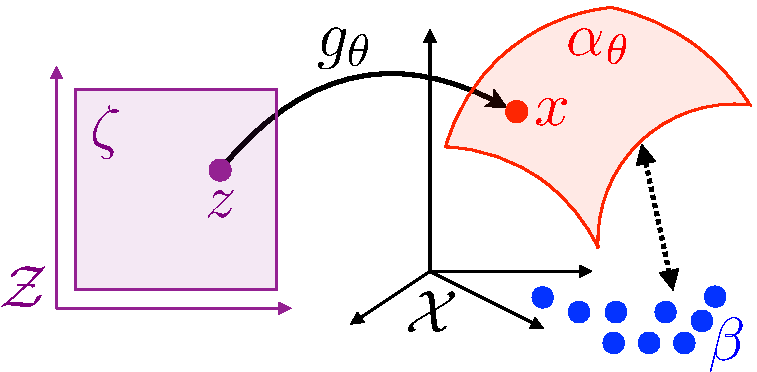
\includegraphics[width=.4\linewidth]{density-fitting/schematic-fitting}
\caption{\label{fig-density-fitting}
Schematic display of the density fitting problem~\ref{eq-density-fitting}.
}
\end{figure}


\newcommand{\fPF}{h}

This MLE approach is known to lead to optimal estimation procedures in many cases (see for instance~\cite{owen2001empirical}). However, it fails to work when estimating singular distributions, typically when the $\al_\th$ does not has a density (so that $\Ll_{\text{MLE}}(\al_\th,\be) = +\infty$) or when $(x_i)_i$ are samples from some singular $\bar\be$ (so that the $\al_\th$ should share the same support as $\be$ for $\KL(\al|\bar\be)$ to be finite, but this support is usually unknown). Another issue is that in several cases of practical interest, the density $\density{\th}$ is inaccessible (or too hard to compute).

A typical setup where both problems (singular and unknown densities) occur is for so-called generative models, where the parametric measure is written as a push-forward of a fixed reference measure $\zeta \in \Mm(\Zz)$
\eq{
	\al_\th = \fPF_{\th,\sharp} \zeta \qwhereq \fPF_\th : \Zz \rightarrow \Xx
}
where the push-forward operator is introduced in Definition~\ref{defn-pushfwd}. The space $\Zz$ is usually low-dimensional, so that the support of $\al_\th$ is localized along a low-dimensional ``manifold'' and the resulting density is highly singular (it does not have a density with respect to Lebesgue measure).
%
Furthermore, computing this density is usually intractable, while generating i.i.d. samples from $\al_\th$ is achieved by computing $x_i=\fPF_\th(z_i)$ where $(z_i)_i$ are i.i.d. samples from $\zeta$.

In order to cope with such difficult scenario, one has to use weak metrics in place of the MLE functional $\Ll_{\text{MLE}}$, which needs to be written in dual form as 
\eql{\label{eq-dual-loss}
	\Ll(\al,\be) \eqdef 
	\umax{(\f,\g) \in \Cc(\X)^2} 
	\enscond{ \int_{\X} \f(x) \d\al(x) + \int_{\X} \g(x) \d\be(x) }{ (\f,\g) \in \Potentials}.
}
Dual norms exposed in~\S\ref{sec-dual-norms} correspond to imposing $\Potentials = \enscond{(\f,-\f)}{\f \in B}$, while optimal transport~\eqref{eq-dual-generic} sets $\Potentials = \Potentials(c)$ as defined in~\eqref{eq-dfn-pot-dual}. 

For a fixed $\th$, evaluating the energy to be minimized in~\eqref{eq-density-fitting} using such a loss function corresponds to solving a semi-discrete optimal transport, which is the focus of Chapter~\ref{c-algo-semidiscr}. Minimizing the energy with respect to $\th$ is much more involved, and is typically highly non-convex.

The class of estimators obtained using $\Ll=\MK_\c$, often called ``Minimum Kantorovitch Estimators'' (MKE), was initially introduced in~\cite{bassetti2006minimum}, see also~\cite{CanasRosasco}. 

% It has been used in the context of generative models by~\cite{CuturiBoltzman} to train Restricted Boltzmann Machines, and in~\cite{bernton2017inference} in conjunction with Approximate Bayesian Computations.  Approximation of these computations using Deep Network are used to train deep generative models for both GAN~\cite{WassersteinGAN} and VAE~\cite{Bousquet2017}, see also~\cite{2017-Genevay-AutoDiff,2017-Genevay-gan-vae}.


%%%%%%%%%%%%%%%%%%%%%%%%%%%%%%%%%%%%%%%%%%%%%%%%%%%%%%%%%%%%%%%%%%%%%%%%%%%%%%%%%%%%
\paragraph{Gromov-Wasserstein.}


Optimal transport needs a ground cost $\C$ to compare histograms $(\a,\b)$, it can thus not be used if the histograms are not defined on the same underlying space, or if one cannot pre-register these spaces to define a ground cost. 
%
To address this issue, one can instead only assume a weaker assumption, namely that one has at its disposal two matrices $\distD \in \RR^{n \times n}$ and $\distD' \in \RR^{m \times m}$ that represent some relationship between the points on which the histograms are defined. A typical scenario is when these matrices are (power of) distance matrices.
%
The Gromov-Wasserstein problem reads
\eql{\label{eq-gw-def}
	\GWD( (\a,\distD), (\b,\distD') )^2 \eqdef
	\umin{ \P \in \CouplingsD(\a,\b) } 
		\Ee_{\distD,\distD'}(\P) \eqdef 
		\sum_{i,j,i',j'} |\distD_{i,i'} - \distD'_{j,j'}|^2 \P_{i,j}\P_{i',j'}.  
}
This is a non-convex problem, which can be recast as a Quadratic Assignment Problem (QAP)~\cite{loiola-2007} and is in full generality NP-hard to solve for arbitrary inputs. 
%
It is in fact equivalent to a graph matching problem~\cite{lyzinski-2015} for a particular cost.

One can show that $\GWD$ satisfies the triangular inequality, and in fact it defines a distance between metric spaces equipped with a probability distribution (here assumed to be discrete in definition~\eqref{eq-gw-def}) up to isometries preserving the measures.
%
This distance was introduced and studied in details by Memoli in~\cite{memoli-2011}. An in-depth mathematical exposition (in particular, its geodesic structure and gradient flows) is given in~\cite{SturmGW}. See also~\cite{schmitzer2013modelling} for applications in computer vision.
%
This distance is also tightly connected with the Gromov-Hausdorff distance~\cite{gromov-2001} between metric spaces, which have been used for shape matching~\cite{memoli-2007,bronstein-2010}. 



%%%%%%%%%%%%%%%%%%%%%
\begin{rem}{Gromov-Wasserstein distance}
	The general setting corresponds to computing couplings between metric measure spaces $(\X,\dist_\X,\al_\X)$
	and $(\Y,\dist_\Y,\al_\Y)$ where $(\dist_\X,\dist_\Y)$ are distances and $(\al_\X,\al_\Y)$ are measures on their respective spaces.
	%
	One defines 
	\begin{align}
		\label{eq-gw-generic}
		\GW( (\al_\X,\dist_\X), (\al_\Y,\dist_\Y) )^2 \eqdef 
		\umin{ \pi \in \CouplingsD(\al_\X,\al_Y) } 
		\int_{\X^2 \times \Y^2}
		| \dist_\X(x,x')-\dist_\Y(y,y') |^2
		\d\pi(x,y)\d\pi(x',y').
	\end{align}
	$\GW$ defines a distance between metric measure spaces up to isometries, where one says that $(\al_\X,\dist_\X)$ and $(\al_\Y,\dist_\Y) $ are isometric if there exists $\phi : \X \rightarrow \Y$ such that $\phi_{\sharp}\al_\X=\al_\Y$ and $\dist_\Y(\phi(x),\phi(x'))=\dist_\X(x,x')$.
\end{rem}
%%%%%%%%%%%%%%%%%%%%%



%%%%%%%%%%%%%%%%%%%%%
\begin{rem}{Gromov-Wasserstein geodesics}
The space of metric spaces (up to isometries) endowed with this $\GW$ distance~\eqref{eq-gw-generic} has a geodesic structure. \cite{SturmGW} shows that the geodesic between  $(\X_0,\dist_{\X_0},\al_0)$ and $(\X_1,\dist_{\X_1},\al_1)$ can be chosen to be 
$t \in [0,1] \mapsto (\X_0 \times \X_1,\dist_t,\pi^\star)$ where $\pi^\star$ is a solution of~\eqref{eq-gw-generic} and for all $((x_0,x_1), (x_0',x_1')) \in (\X_0 \times \X_1)^2$, 
\eq{
	\dist_t((x_0,x_1), (x_0',x_1')) \eqdef
	(1-t)\dist_{\X_0}(x_0,x_0') + t\dist_{\X_1}(x_1,x_1').
}
This formula allows one to define and analyze gradient flows which minimize functionals involving metric spaces, see~\cite{SturmGW}. It is however difficult to handle numerically, because it involves computations over the product space $\X_0 \times \X_1$. 
%
A heuristic approach is used in~\cite{peyre2016gromov} to define geodesics and barycenters of metric measure spaces while imposing the cardinality of the involved spaces and making use of the entropic smoothing~\eqref{eq-gw-entropy} detailed below.
\end{rem}
%%%%%%%%%%%%%%%%%%%%%

To approximate the computation of $\GWD$, and to help convergence of minimization schemes to better minima, one can consider the entropic regularized variant
\eql{\label{eq-gw-entropy}
	\umin{ \P \in \CouplingsD(\a,\b) } 
		\Ee_{\distD,\distD'}(\P) - \epsilon \HD(\P).
}
As proposed initially in~\cite{gold-1996,rangarajan-1999}, and later revisited in~\cite{2016-solomon-gw} for applications in graphics, one can use iteratively Sinkhorn's algorithm to progressively compute a stationary point of~\eqref{eq-gw-entropy}. 
%
Indeed, successive linearizations of the objective function lead to consider the succession of updates
\eql{\label{eq-gw-sinkh}
	\itt{\P} \eqdef \umin{ \P \in \CouplingsD(\a,\b) } \dotp{\P}{\it{\C}} - \epsilon\H(\P)
		\qwhereq
}
\eq{
		\it{\C} \eqdef \nabla \Ee_{\distD,\distD'}(\it{\P}) = -\transp{\distD'} \it{\P} \distD, 
}
which can be interpreted as a mirror-descent scheme~\cite{2016-solomon-gw}. Each update can thus be solved using Sinkhorn iterations~\eqref{eq-sinkhorn} with cost $\it{\C}$. Figure~\eqref{fig-gw} illustrates the use of this entropic Gromov-Wasserstein to compute soft maps between domains. 


\begin{figure}
\centering
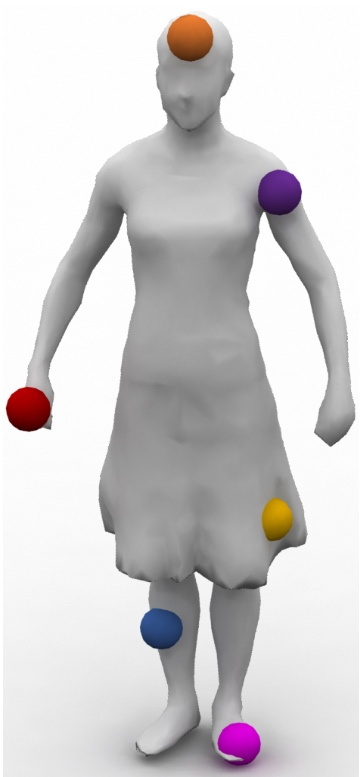
\includegraphics[height=.22\linewidth]{gw/source}
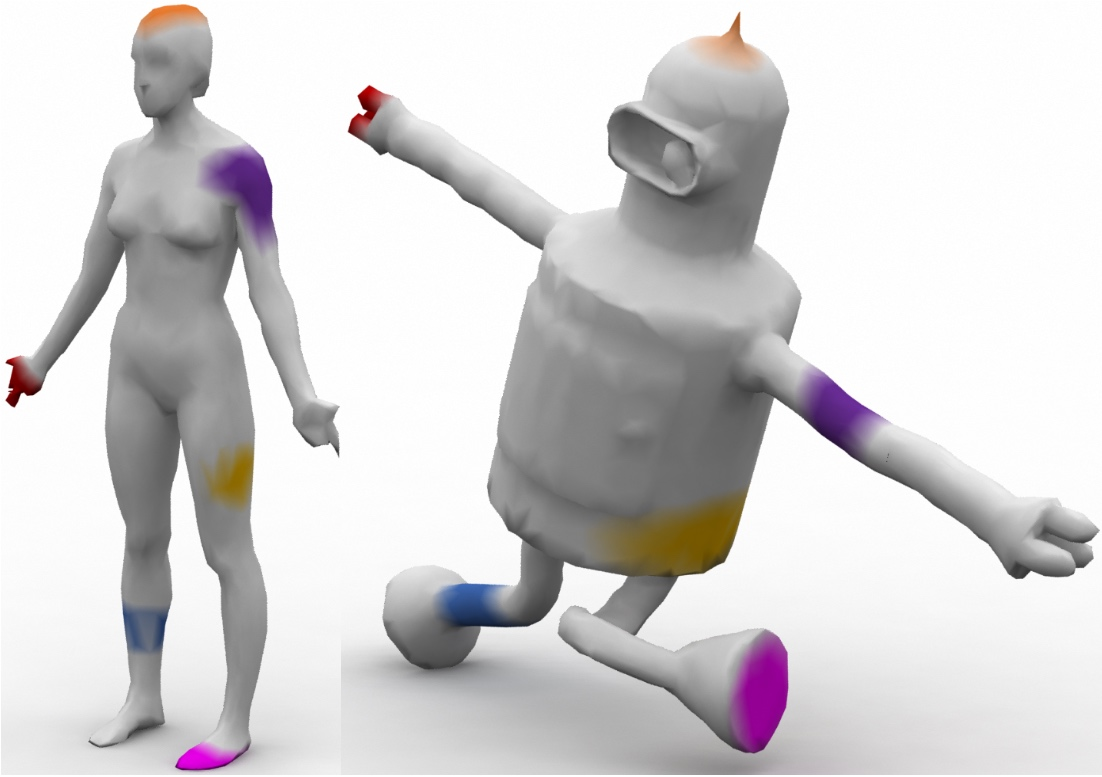
\includegraphics[height=.22\linewidth]{gw/target-surf}
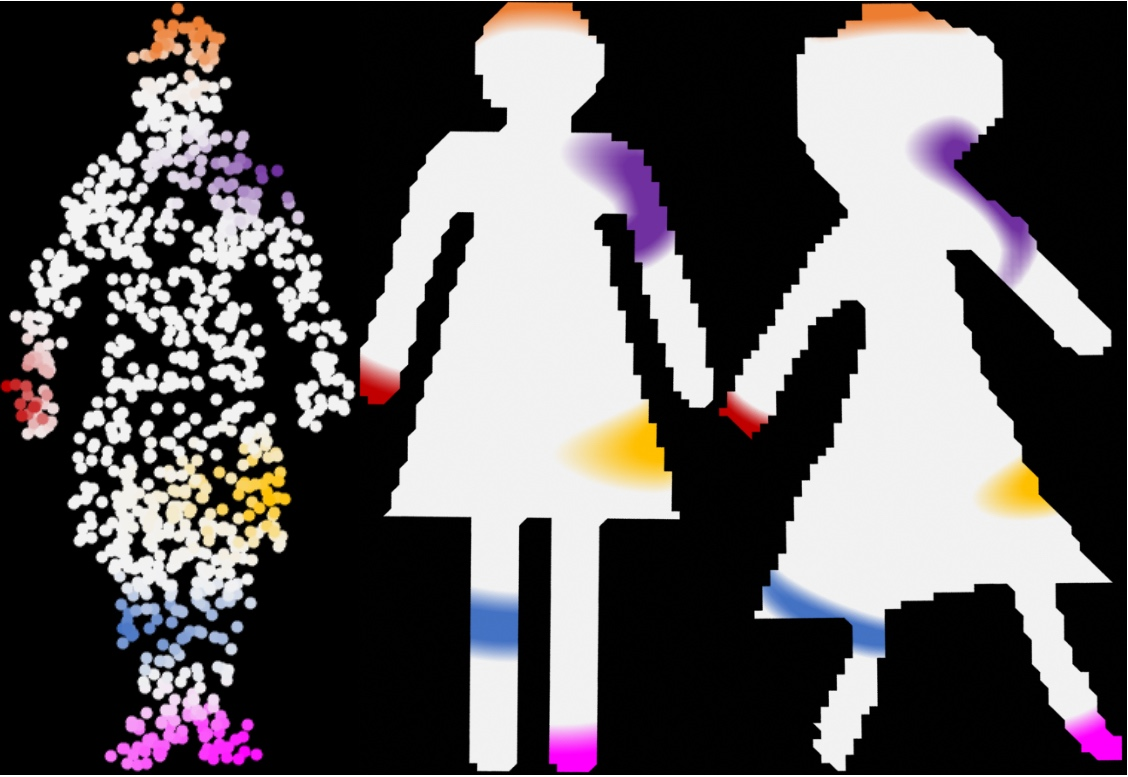
\includegraphics[height=.22\linewidth]{gw/target-2d}
\caption{\label{fig-gw}
Example of fuzzy correspondences computed by solving GW problem~\eqref{eq-gw-entropy} with Sinkhorn iterations~\eqref{eq-gw-sinkh}. Extracted from~\cite{2016-solomon-gw}.
}
\end{figure}

